\documentclass[11pt]{amsart}


\newtheorem{theorem}{Theorem}[section]
\newtheorem{lemma}[theorem]{Lemma}
\newtheorem{corollary}[theorem]{Corollary}
\newtheorem{proposition}[theorem]{Proposition}
\newtheorem{noname}[theorem]{}
\newtheorem{sublemma}{}[theorem]
\newtheorem{conjecture}[theorem]{Conjecture}

\theoremstyle{definition}
\newtheorem{definition}[theorem]{Definition}
\newtheorem{example}[theorem]{Example}

\theoremstyle{remark}
\newtheorem{remark}[theorem]{Remark}
\newtheorem{claim}{Claim}

\numberwithin{equation}{section}

\newcommand{\ba}{\backslash}
\newcommand{\utf}{uniform time function}

\usepackage{fullpage}
\usepackage{graphicx}
\usepackage{amssymb}
\usepackage{amsmath}
\usepackage{enumerate}
\usepackage{amstext}
\usepackage{verbatim}

\begin{document}

\title[Growth of Groups Defined by Automata]{Growth of Groups Defined by Automata}


\author{Ashley S. Dougherty}
\address{ 
	(Dougherty)
	Department of Education,
	Department of Mathematics,
  Kutztown University
	Kutztown, PA 19530
	gffadougherty@yahoo.com
	}

\author{Lydia R. Kindelin}
\address{
        (Kindelin)
        Department of Mathematics,
        University of Dayton,
        Dayton, OH 45302
        kindelinl1@notes.udayton.edu 
         }

\author{Aaron M. Reaves}
\address{
	(Reaves)
	Department of Mathematics,
	Morehouse College,
	Atlanta, GA 30314
	reavesam@gmail.com
	}
	
\author{Andrew J. Walker}
\address{
        (Walker)
        Department of Physical Sciences,
        York College of Pennsylvania,
        York, PA 17403
        awalker6@ycp.edu 
        }

\author{Nathaniel F. Zakahi}
\address{
	(Zakahi)
        Department of Mathematics and Computer Science,
        Denison University,
        Granville, OH 43023
        zakahi\_n@denison.edu
	}




\begin{abstract}
Nekrashevych conjectured that iterated monodromy groups of quadratic polynomials with a pre-periodic kneading sequence have intermediate growth. In this paper we prove intermediate growth for two such groups. We also provide a new proof of intermediate growth for a class of groups containing the Grigorchuk group, previously known to have intermediate growth.
\end{abstract}



\maketitle{}

%%%%%%%%%%%%%%%%Starts Here%%%%%%%%%%%%%%%%%%%%%%%%%%%%%%%%%%%%%%%%%%%%%%%%%%%%%%%%%%%%%%%%%%%%%%%%


\section{Introduction}

\indent Finitely generated groups of infinite order grow at many different rates. Growth functions are more commonly polynomial or exponential but there are rarer cases of intermediate growth. Grigorchuk found the first group of intermediate growth in the 1980's and these groups have been studied ever since.\\
\indent Grigorchuk's group is generated by an automaton and these mathematical structures are convenient for finding groups of intermediate growth. Nekrashevych provides a process in his monograph \textit{Self-Similar Groups} for producing an automaton from any given post-critically finite polynomial. He also conjectured that a specific kind of post-critically finite polynomial would produce an automaton which would generate a group of intermediate growth. We have considered this conjecture and found two more groups of intermediate growth using Nekrashevych's procedure.\\
\indent The automata produced by Nekrashevych's process are of a specific form and the Grigorchuk group does not come from such an automaton. We looked at automata with similar properties to that of the Grigorchuk group and give a new proof that a known class of automata will produce groups of intermediate growth.\\
\indent In order to prove intermediate growth of groups we modeled our arguments on those from the paper \textit{On the Growth of Iterated Monodromy Groups} Bux and P\'{e}rez \cite{BuxP} with the use of a weight system to represent the length of words. This method can be used to prove intermediate growth for both, groups produced by polynomials in Nekrashevych's process, and groups generated by any automaton. In this paper we also discuss some of the obstacles we encountered with this method for proving intermediate growth.
\newpage

\section{Background}

\subsection{Growth}

\begin{definition} 
\indent For a finite generating set $\Sigma$ of a group $G$ and a map $\tilde{\ell}: \Sigma\to \mathbb{R}^+$, the \textit{ball of radius} $\mathit{n}$, $B_G(n)$ is the set of all elements $g\in G$ represented by a word $w=x_1^{\epsilon_1}x_2^{\epsilon_2}\cdots x_m^{\epsilon_m}$, $x_i\in \Sigma$, $\epsilon_i=\pm 1$, with $\displaystyle \sum_{i=1}^n\tilde{\ell}(i)\leq n$.\end{definition}
\begin{definition}
\indent The \textit{growth function} $g(n): \mathbb{N}\to \mathbb{N}$ of $G$ is defined by $g(n)=|B_G(n)|$.\\
\end{definition}


\begin{definition}
Let $f,g\in \mathbb{N}\cup \left\{0\right\} \rightarrow \mathbb{N}\cup \left\{0\right\} $. We say that $f\preceq g$ if there are constants $A,B,C \in \mathbb{N}$ such that $f(n)\leq Ag(Bn)+C$, for all $n \in \mathbb{N} \cup \left\{0\right\}$.
\end{definition}

\begin{definition}
Let $G$ be a group with the finite generating set $S$ and growth function $g(n)$.  We say $G$ has \textit{polynomial growth} if there exists some polynomial $p(n)$ such that $g(n)\preceq p(n)$.  We say $G$ has \textit{exponential growth} if there exists some $a> 1$ such that $a^n\preceq g(n)$. A group $G$ has \textit{intermediate growth} if $p(n)\preceq g(n) \preceq a^n$ for all polynomials $p$ and some $a > 1$. Growth is not dependent on the generating set but is a property of the group in general.
\end{definition}




\subsection{Automata}

\subsubsection{Defining Automata}

\indent Except for the definition of the infinite rooted $n$-ary tree, the following definitions come from Nekrashevych
{Nekr}. The tree definition is general knowledge; our definition comes from Terpstra\cite{Terp}.

\begin{definition}
For an integer $n \geq 2$ define $\mathcal{T}^n$ to be the \textit{infinite rooted $n$-ary tree}. The vertices of $\mathcal{T}^n$ are finite sequences of elements (or possibly $\emptyset$) from $\{0,1,\ldots,n - 1\}$, and the edges of $\mathcal{T}^n$ connect pairs of vertices whose sequences differ in length by $1$, and in which the shorter sequence can be obtained by erasing the last term of the longer sequence. For example, vertices $v_i = (011)$ and $v_j = (0110)$ would be connected by an edge, while $v_l = (010)$ and $v_j=(0110)$ would not. The empty sequence defines the \textit{root} vertex denoted by $\emptyset$.
\end{definition}

\begin{definition}
Let $\Gamma$ be a simple graph. An \textit{automorphism} of $\Gamma$ is a bijection of the vertices that preserves the adjacency and non-adjacency. 
\end{definition}

\begin{definition}
An \textit{alphabet} is a set $\textsf{X}$. The \textit{free monoid on $\textsf{X}$}, denoted $\textsf{X*}$, is the set (possibly empty) of all $n$-tuples.
\end{definition}

\begin{definition}    
An \textit{automaton} $\textsf{A}$ over the alphabet $\textsf{X}$ is given by
\begin{enumerate}
\item a \textit{set of the states}, usually also denoted by $\textsf{A}$
\item a map $\tau : \textsf{A}\times \textsf{X} \rightarrow \textsf{X}\times \textsf{A}$
\end{enumerate}
\end{definition}

\begin{definition}
It is convenient to define automata using their \textit{Moore diagrams}. A Moore diagram is a directed labeled graph with the vertices identified with the states of the automaton. If $\tau(q \cdot x) = y \cdot p$, then we write $q\cdot x=y\cdot p$, and we have an arrow starting in $q$, ending in $p$ and labeled by $(x,y)$. So, the arrows show the state transitions, and their labels show the input and the output.
\end{definition}

\subsubsection{Groups Generated by Automata}\text{\space} The group generated by the automaton $\textsf{A}$ is the group $\left\langle \textsf{A} \right\rangle$ generated by the transformations defined on all the states of $\textsf{A}$.\\

\indent For example, consider the automaton $\textsf{A}$ over the alphabet $\textsf{X}$ containing state $q$. Then $q$ is represented by an $n$-tuple where the first coordinate represents how the state acts with $0$, the second coordinate is how the state acts with $1$, and so on through $n - 1$ actions. So, if $q \cdot 0 = 0 \cdot p$ and $q \cdot 1 = 1 \cdot r$, then $q = (p,r)$. This bracket notation means that when the state $q$ acts on the $n$-ary tree, it does nothing to the $0$ but produces a $p$ at the next vertex of the tree and does nothing to $1$ but produces an $r$ at the next vertex. This notation is also an easier way to multiply elements of the group. If $q = (p,r)$ and $p = (1,q)$ then $qp = (p,r)(1,q) = (p,rq)$. Another important aspect of the bracket notation is the ease in representing certain automorphisms of the tree. Consider an automorphism $\alpha := (\alpha_L, \alpha_R) \in Aut(T^{(2)})$ where $\alpha$ preserves each of the two subtrees and acts in $T_{L}^{(2)}$ as $\alpha_L$ and in $T_{R}^{(2)}$ as $\alpha_R$. Now, consider $\tau \in Aut(T^{(2)})$, called the swap, that interchanges $T_{L}^{(2)}$ and $T_{R}^{(2)}$. So, $\tau (\alpha_L,\alpha_R) = (\alpha_R,\alpha_L) \tau$. For $\tau \in Aut(T^{(3)})$, $\tau(\alpha_L,\alpha_C,\alpha_R) = (\alpha_R,\alpha_L,\alpha_C)\tau$.\\

\subsubsection{Nekrashevych's Process for Creating Groups from Polynomials}

\begin{definition}
An \textit{active state} $a$ of an automaton $A$ is a state such that $a\times x\to y\times a$ for some $x\neq y\in \textsf{X}$. Because of this, a state in an automaton may be seen as a string transformation on strings of the alphabet, with an active state $a$ transforming $x$ to $y$ and a non-active state as the identity transformation.
\end{definition}

\begin{definition}
For an automaton $\textsf{A}$ with only a single active state and a single arrow leading to and from each non-active state that does not go to the identity state, the \textit{kneading sequence} of $\textsf{A}$ is the sequence of $x_i\in X$ labeling the arrows not leading to the identity state. The first arrow, with corresponding $x_1$ is the arrow entering the active state, and each successive arrow is the arrow entering the state the previous arrow began at. A \textit{periodic kneading sequence} is when the kneading sequence is a loop connecting all the labels of the arrows of the Moore diagram. A \textit{pre-periodic kneading sequence} is when the kneading sequence has a straight path for at least one action and then is a loop connecting the rest of the labels.
\end{definition}

\begin{definition}
Let $p:\mathbb{C}\rightarrow\mathbb{C}$ be a complex polynomial such that $p(z)=a_z^n+a_{n-1}z^{n-1}+\cdots a_1z+a_0$. A \textit{critical point} of the polynomial is a solution of $p'(z)=0$.  A \textit{post-critical point} is a point $p(p(p(\ldots(c))))$ where $c$ is a critical point.  We say that $p$ is \textit{post-critically finite} if the set $P$ of all post-critical points is finite. 
\end{definition}


In Nekrashevych's monograph, \textit{Self-Similar Groups}, he provides a process for constructing automata from post-critically finite polynomials. These automata can be used to define iterated monodromy groups. We only describe the process for finding these groups, but a thorough discussion of them can be found in the monograph \cite{Nekr}. It is important to note that for any post-critically finite polynomial $f : \mathbb{R}^2 \rightarrow \mathbb{R}^2$, if there exists an $f$-invariant spider as defined below, there will always exist an automaton which generates the action of IMG$(f)$.

\begin{conjecture}
Nekrashevych conjectured that every second degree post-critically finite polynomial with a pre-periodic kneading sequence produces an iterated monodromy group of intermediate growth.\\
\end{conjecture}


\begin{definition}
A \textit{spider} $\mathcal{S}$ is a collection of disjoint simple curves in the complex plane connecting each of the post-critical points to infinity (since the number of post-critical points is finite, a spider will always exist). For each $z\in P$, we call the curve connecting $z$ to infinity $\gamma_z$. Each curve $\gamma_z$ may not pass through any post-critical points other than its initial point at $z$. A spider $\mathcal{S}$ is said to be $f-invariant$ if $f(\mathcal{S})$ is isotopic to a subset of $\mathcal{S}$ through spiders.\end{definition}
\begin{definition}
\indent For a critical point $z\in C$ of local degree $d_z$, the set $X_z=f^{-1}(\gamma_{f(z)})$ consists of $d_z$ curves connecting $z$ to infinity. The collection $\{X_z \mid z\in C\}$ of such sets of curves is called the \textit{critical portrait} associated to the spider $\mathcal{S}$ and the topological polynomial. The curves of the critical portrait will divide the plane into components, called \textit{sectors}.
\end{definition}



\indent For a polynomial $f$ with a finite post-critical set and corresponding $f$-invariant spider $\mathcal{S}$, there will exist some critical portrait, $\mathcal{C}$. Then let $\{S_x \mid x\in \textsf{X}\}$ be the set of corresponding sectors, where \textsf{X}, with $|\textsf{X}|=d$, is the set of labels of the sectors.\\
\indent We shall construct the automaton $K_{\mathcal{C},f}$ using \textsf{X} as our alphabet. We label this automaton $K_{\mathcal{C},f}$, as it encodes both the critical portrait $\mathcal{C}$ and the action of the polynomial $f$. The procedure is as follows:\\


\begin{enumerate}

\item[Part A] Take an arbitrary post-critical point $z\in P$. For each $y\in f^{-1}(z)$, if $y$ is not critical, proceed to Part B. Otherwise, skip to Part C.\\
\item[Part B] As $y$ is not critical, the local degree of $f$ around $y$ should be $1$, and $y$ should be an internal point of a sector $S_x$. This information will be encoded by the output and transition functions of $K_{\mathcal{C},f}$: $$g_z\cdot x=x\cdot g_y,$$
where $g_y=id$ if $y\notin P$.\\
\item[Part C] Since $y$ is critical, it will be on the boundaries of $d'$ sectors. Let these sectors be $S_{x_1},S_{x_2},S_{x_3},\ldots S_{x_{d'}}$, listed in counterclockwise order around $y$. The set $\mathsf{X}$, which we already defined as the set of labels of the sectors, will then be the set $\{x_1, x_2,x_3,\ldots x_{d'}\}$. If $y$ is not post-critical, go to Part C-I. If it is post-critical , go to part C-II.\\
\item[Part C-I] Since $y$ is not post critical, we encode the action of a small loop around $y$ by setting: $$g_z\cdot x_i=x_{i+1 (\textmd{mod } d')}\cdot id$$ for $i=1,\ldots d'$.\\
\item[Part C-II] Since $y$ is post-critical, there is a path $\gamma_y$ in the spider $\mathcal{S}$. We may assume the sectors are labeled in such a way that the curve $\gamma_y$ is adjacent to $S_{x_1}$ and $S_{x_{d'}}$. Let us then encode this by $$g_z\cdot x_i=x_{i+1}\cdot id$$ for $i=1,\ldots,d'-1$ and $$g_z\cdot x_{d'}=x_1\cdot g_y.$$\\

Once this process has been completed for every post-critical point in the set $P$, we can draw the corresponding Moore diagram.\\

\end{enumerate}


\section{Computations of Iterated Monodromy Groups of Polynomials}
\indent In this section, we compute the iterated monodromy groups for the polynomials $z^2-2$, $z^3+3z$, $z^3-3z$, and $z^3+\frac{3}{2}z$. We then show they are all of polynomial growth in Proposition \ref{Poly}.\\

\subsection{The Iterated Monodromy Group of $\mathbf{p(z)=z^2-2}$} \text{\space}\\
\indent Here, we use a simple example to demonstrate Nekrashevych's procedure for producing iterated monodromy groups. Consider the polynomial $z^2 - 2$. The derivative of $z^2 - 2$ is $2z$, and when set equal to zero, $z$ must equal zero. Therefore, the set of critical points, $C$, only contains $0$. When we substitute $0$ into $z^2 - 2$ for $z$, we get $-2$. When $-2$ is similarly substituted back into the polynomial, we get $2$, and $2$ will always produce another $2$ when substituted for $z$. Therefore, the set of post-critical points is $P = \{-2,2 \}$ and $z^2 - 2$ is post-critically finite. Now we will construct the spider $\mathcal{S}$. Let $$\gamma_{-2} = \{z \in \mathbb{C} \mid z = -2 + it, t \in \mathbb{R^+} \cup \{0\} \},$$ $$\gamma_2 = \{z \in \mathbb{C} \mid z = 2 - it, t \in \mathbb{R^+} \cup \{0\} \}$$ portrayed in the picture below where $$f(\gamma_{-2}) = \{z\in \mathbb{C} \mid (2 - t^2 - 4it), t \in \mathbb{R^+} \cup \{0\} \},$$ $$f(\gamma_2) =\{z\in \mathbb{C} \mid (2 - t^2 - 4it),t \in \mathbb{R^+} \cup \{0\} \}$$.\\

\begin{center}
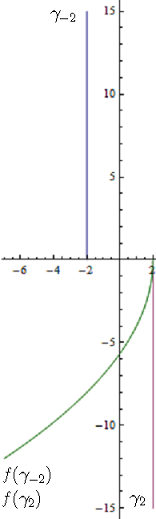
\includegraphics[scale=0.5]{z2minus2spider.png}
\end{center}

\indent To obtain the line $X_0$ and complete the critical portrait, we set $X_0 = f^{-1}(\gamma_{f(0)})$. Then, $f^{-1}(\gamma_{f(0)}) = f^{-1}(\gamma_{-2}) = \{z \in \mathbb{C} \mid f(z) = -2 + it, t \in \mathbb{R^+} \cup \{0\} \}$. Thus:
\begin{align*}
& z^2 - 2 = -2 + it\\
& z^2 = it\\
& z^2 = te^{\frac{\pi}{2}i}\\
& te^{\frac{\pi}{2}i} = r^2e^{2\theta i}\\
& r^2 = t\\
& 2\theta = \frac{\pi}{2} + 2\pi n, n \in \mathbb{Z}\\
& \theta = \frac{\pi}{4} + \pi n\\
\end{align*}

\indent The last step in labeling the critical portrait is to determine which sector is $S_0$ and which is $S_1$. We want to label the sectors starting with $S_0$ and moving counterclockwise around $X_0$ to label $S_1$. Since we only have two sectors, one valid labeling of the graph is as follows:\\

\begin{center}
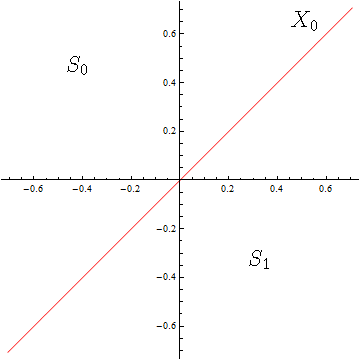
\includegraphics[scale=0.5]{z2minus2criticalportrait.png}
\end{center}

\indent Let the post-critical points $-2$ and $2$ be represented by $a$ and $b$ respectively. This gives our set of states $A = \left\{a,b,id\right\}$ and our alphabet $\textsf{X} = \left\{0,1\right\}$.\\
\indent Now let $z$ be the post-critical point $-2$. Then $y = f^{-1}(z) = 0$. Note $0$ is not a post-critical point, but since it is a critical point, it lies on $X_0$. Thus, we set $a \cdot 0 = 1 \cdot id$ and $ a \cdot 1 = 0 \cdot id$ as defined by $g_z \cdot x_i = x_{i+1 (\textmd{mod } d')} \cdot 1$ for $i = 1,\ldots,d'$ where $S_{{x}_{d'+1}} = S_{{x}_{1}}$. Consider next the other post-critical point $2$. Then $f^{-1}(z) = \left\{-2,2\right\}$. Thus, we must finish the procedure for both $y=2$ and $y=-2$. For $y = 2$, since $2$ is not a critical point and lies in $S_1$, we obtain $b \cdot 1 = 1 \cdot b$ by applying $g_z \cdot x = x \cdot g_y$ where $g_y = 1$ if $y \notin P$. For $y = -2$, we apply the same formula, with the exception that $-2$ lies in $S_0$. This gives $b \cdot 0 = 0 \cdot a$. These actions give the following automaton:\\

\begin{center}
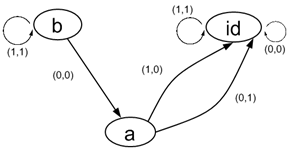
\includegraphics{z_2.png}
\end{center}

\indent We may also represent the actions of each state of the automaton in bracket notation. The state $a$ acts as the transposition $(01)$, which we commonly refer to as $\tau$. The state $b$ will act differently on 0 and 1, but it does not change the number in either case. When it acts on a $0$, it returns the 0 and goes to $a$, and when it acts on a $1$, it returns the 1 and goes back to itself. Therefore $b = (a,b)$.

\subsection{The Iterated Monodromy Group of $\mathbf{p_1(z)=z^3+3z}$} \text{\space}\\

\indent A more interesting example comes from the polynomial $p_1(z) = z^3 + 3z$.  Carrying out the same procedure explained earlier, we find $C = \{i, -i\}$ and $P = \{2i, -2i\}$. We may then create the following spider with $\gamma_{2i} =\{z \in \mathbb{C} \mid z =  2i-t, t \in \mathbb{R^+}\}$ and $\gamma_{-2i} = \{z \in \mathbb{C} \mid z =  t-2i, t \in \mathbb{R^+}\} $.\\

\begin{center}
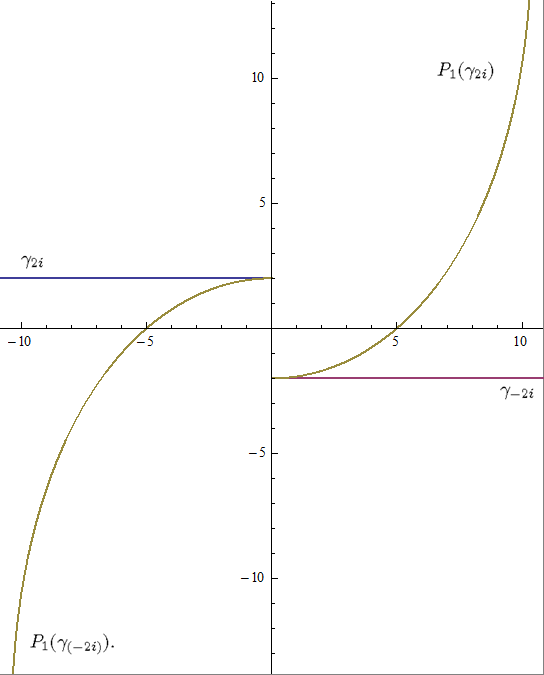
\includegraphics[scale=0.4]{plus_3z_spider.png}
\end{center}

We may note it is a $p_1$-invariant spider, with $p_1(\gamma_{2i})$ and $p_1(\gamma_{(-2i)})$ also depicted. We also give the critical portrait, with $X_{(i)}$ and $X_{(-i)}$ depicted.\\

\begin{center}
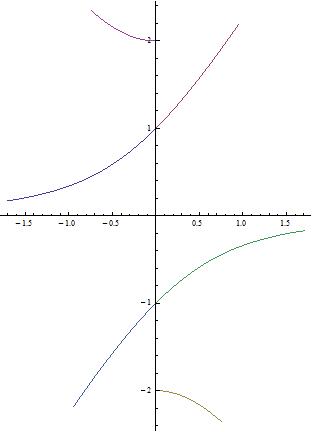
\includegraphics[scale=0.5]{plus3zcritical.png}
\end{center}

\indent  We assign the post critical points $2i$ and $-2i$ to the states $a$ and $b$, respectively, and we the find the actions to be:
$a \cdot 0 = 1 \cdot id, a \cdot 1 = 0 \cdot id, a \cdot 2 = 2 \cdot b$ and $b \cdot 0 = 0 \cdot a, b \cdot 1 = 2 \cdot id, b \cdot 2 = 1 \cdot id$.\\
\indent We then have our final automaton, with its Moore diagram depicted here: 

\begin{center}
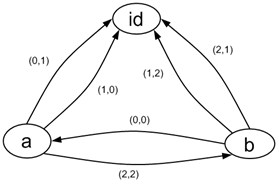
\includegraphics{z_33z.png}
\end{center}

\indent We may then convert the automaton into a group with the previously introduced bracket notation. This gives group elements $a = \alpha(1, 1, b)$ and $b = \beta(a, 1, 1)$, where $ \alpha = (0 1)$ and $\beta = (1 2)$.  

\subsection{The Iterated Monodromy Group of $\mathbf{p_2(z)=z^3-3z}$} \text{\space}


\indent A similar example is the iterated monodromy group of $p_2(z) = z^3 - 3z$.  Following the same procedure, we have $C = \{1, -1\}$ and $P = \{-2, 2\}$. We may graph $\gamma_{2}(t) = 2 + ti$, $\gamma_{-2}(t) = -2 - ti$, along with $p_2(\gamma_{2})$ and $p_2(\gamma_{(-2)})$ to create a $p$-invariant spider, figure.\\

\begin{center}
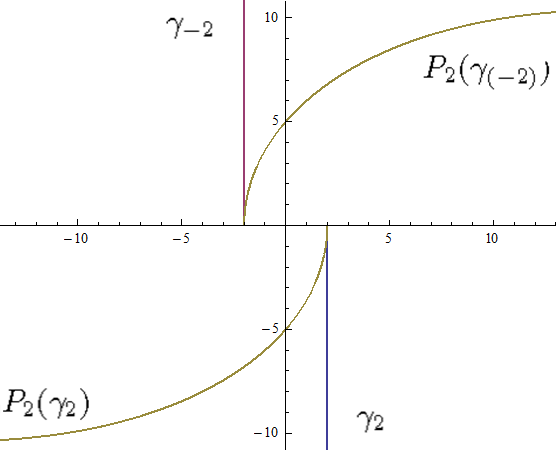
\includegraphics[scale=0.5]{minus_3_spider2.png}
\end{center}

The curves $X_{(1)}$ and $X_{(-1)}$ are graphed to form the critical portrait shown below.\\

\begin{center}
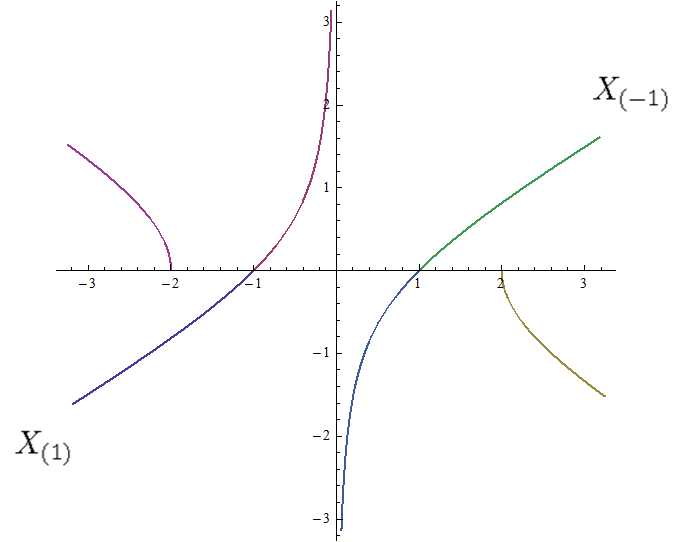
\includegraphics[scale=0.5]{minus3critical2.png}
\end{center}

\indent This critical portrait leads to the following actions of the group elements $a$ and $b$.  With $a$ labeling post critical point $2$ and $b$ labeling $-2$, the actions of the group are:
$a \cdot 0 = 1 \cdot id, a \cdot 1 = 0 \cdot id, a \cdot 2 = 2 \cdot a$ and $b \cdot 0 = 0 \cdot b, b \cdot 1 = 2 \cdot id, b \cdot 2 = 1 \cdot id$.  Here we show the automaton:

\begin{center}
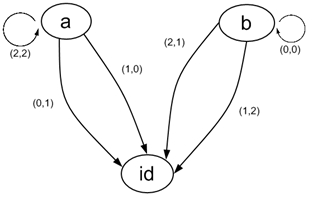
\includegraphics{z_3_3z.png}
\end{center} 

\indent In bracket notation, these group elements are represented as $a = \alpha(1, 1, a)$ and $b = \beta(b, 1, 1)$, where $\alpha$ and $\beta$ are cycles $ \alpha = (0 1)$ and $\beta = (1 2)$.  



\subsection{The Iterated Monodromy Group of $\mathbf{p_3(z)=z^2+\frac{3}{2}z}$} \text{\space}

\indent For a final example, we use the post-critical polynomial $p_3(z)= z^3 + \frac{3}{2}z$. For this polynomial we have $C = \{ \frac{i}{\sqrt{2}},\frac{-i}{\sqrt{2}}\}$ and  $P = \{ p_3 (\frac{i}{\sqrt{2}}),p_3 (\frac{-i}{\sqrt{2}})\}$.  We may note having $p_3$ act on either of the critical points simply returns that point, that is, $p_3(\frac{i}{\sqrt{2}}) = \frac{i}{\sqrt{2}}$ and $ p_3(\frac{-i}{\sqrt{2}}) = \frac{-i}{\sqrt{2}}$.\\
\indent As described earlier, we chose the curves, $\gamma_{(\frac{i}{\sqrt{2}})} = \{z \in \mathbb{C} \mid -t + \frac{i}{\sqrt{2}} : t \geq 0\}$ and $\gamma_{(\frac{-i}{\sqrt{2}})} = \{z \in \mathbb{C} \mid t - \frac{i}{\sqrt{2}} : t \geq 0\}$ to construct the $f$-invariant spider $p_3(\gamma_{(\frac{i}{\sqrt{2}})})$ and $p_3(\gamma_{(\frac{-i}{\sqrt{2}})})$.\\

\begin{center}
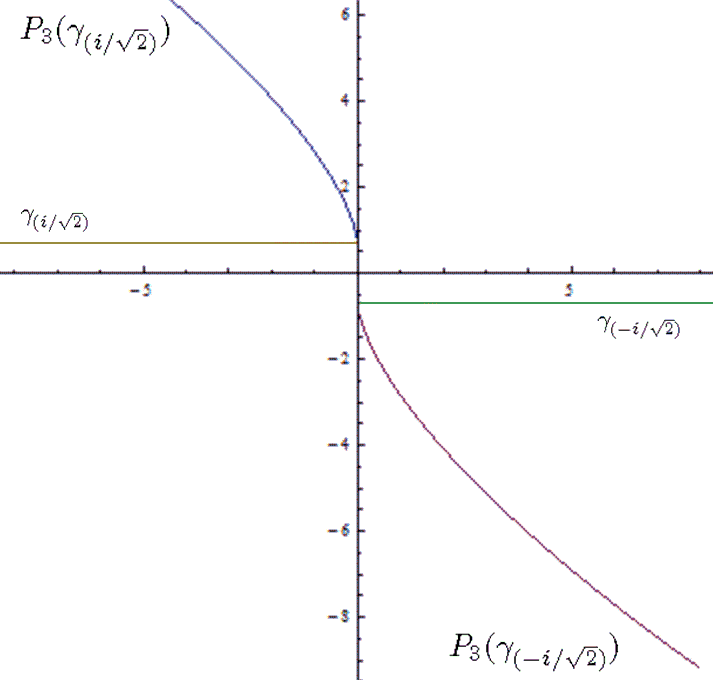
\includegraphics[scale=0.25]{1_5_spider_2.png}
\end{center}

\indent Again, we wish to create a critical portrait for the polynomial with the set of curves $X_z = \{{p_3}^{-1}(\gamma_{(P_3(z))}) \mid z \in C\}$.  Therefore our critical portrait contains two curves $X_{(\frac{i}{\sqrt{2}})}$ and $X_{(\frac{-i}{\sqrt{2}})}$ and below is the critical portrait we constructed.\\

\begin{center}
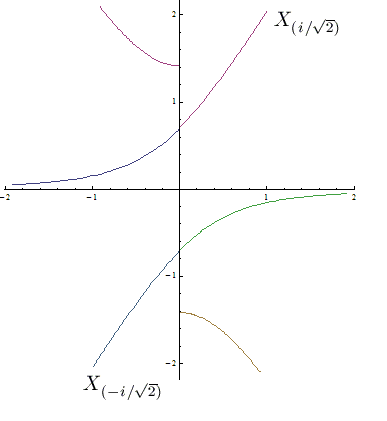
\includegraphics[scale=0.5]{1_5critical1.png}
\end{center} 

\indent This critical portrait is different than those other polynomials because its critical points are the same as its post-critical points. This causes both post-critical points lie on the curves of the critical portrait.\\

\indent State $a$ corresponds to the post critical point $\frac{i}{\sqrt{2}}$ and state $b$ corresponds to the post critical point $\frac{-i}{\sqrt{2}}$. The group actions are for $a$ are $a \cdot 0 = 1 \cdot a, a \cdot 1 = 0 \cdot id, a \cdot 2 = 2 \cdot id$, and the actions for $b$ are $b \cdot 0 = 0 \cdot id, b \cdot 1 = 2 \cdot b, b \cdot 2 = 1 \cdot id$. The following automaton represents the group of automorphisms from this polynomial:

\begin{center}
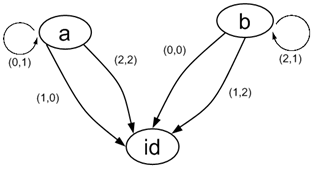
\includegraphics{z_32z.png}
\end{center} 

\indent Note $ \alpha = (0 1)$ and $\beta = (1 2)$. Thus, writing $a$ and $b$ in bracket notation gives $a = \alpha(a, 1, 1)$ and $b = \beta(1, b, 1)$.\\


\subsection{Isomorphism with the Infinite Dihedral Group}

\begin{proposition} \label{Poly}
\indent The iterated monodromy groups of $p,p_1,p_2$, and $p_3$ have polynomial growth. 
\end{proposition}

\indent For the proof, we shall show the iterated monodromy group of $z^3-3z$ is isomorphic to $D_\infty$, which is a group known to have polynomial growth. The other groups proofs are similar.\\

\begin{proof} 
\indent First, note that both $\alpha$ and $\beta$ have order two, as they are simple transpositions of two letters of our alphabet. Next, we show both $a$ and $b$ are also of order 2. Taking advantage of the bracket notation, we see $a^2 = \alpha(1, 1, b)\alpha(1, 1, b)=(1,1,b^2).$\\
\indent However, we can also show this explicitly through acting on strings of the alphabet, considering $\alpha(1, 1, b)\alpha(1, 1, b)(x_1 x_2 x_3 \ldots  x_n)$ for some ternary string $x_1x_2\ldots x_n$. If $x_1$ is either $0$ or $1$, then, $(1,1,b)$ simply acts as the identity, and since $\alpha$ acts on $x_1$ twice, it also does nothing, and, we simply find $$\alpha(1, 1, b)\alpha(1, 1, b)(x_1 x_2 x_3 \ldots x_n) = \alpha(1, 1, b)\alpha (1) (x_1 x_2 x_3 ... x_n) = (x_1 x_2 x_3 ... x_n).$$ 
\indent On the other hand, if $x_1 = 2$, then $(1,1,b)$ acts as the identity on $x_1$ and as $b$ on $x_2x_3\cdots x_n$, but $\alpha$ acts as the identity on $x_1$, as it does not permute 2. Thus, $$\alpha(1, 1, b)\alpha(1, 1, b)(2 x_2 x_3 \ldots x_n) = \alpha(1, 1, b)2 b (x_2 x_3 \ldots  x_n) = 2 b^2(x_2 x_3 \ldots  x_n).$$ Therefore, we again find $a^2 = (1,1,b^2)$.\\
\indent Using a similar process, we find $b^2 = \beta(a, 1, 1)\beta(a, 1, 1) = (a^2, 1, 1)$. Applying this inductively, we may note neither $a^2$ nor $b^2$ will ever contain an active state in any of their terms, and they will thus never act non-trivially on any string. Thus, they are both the identity, giving $a$ and $b$ each order 2.\\

\indent Next, we will show the group element $ab$ and its inverse $ba$ are each of infinite order. To show this, we will assume the contrary, they are of finite order.\\
\indent For this, note, $ab = \alpha(1, 1, b)\beta(a, 1, 1)$. Again taking advantage of bracket notation, this gives $ab=\alpha\beta(1,b,1)(a,1,1)=\alpha\beta(a,b,1)$. Similarly, $ba=\beta\alpha(1,a,b)$.\\ 
\indent Note $\alpha\beta=(012)$ and $\beta\alpha=(210)$. Thus, both of these are of order 3, as they are cycles of three elements. Since $\alpha\beta$ is the only part of $ab$ not fixing the top branch of the tree, we may then note the order of $ab$ must also be a multiple of 3, else the top branch will have changed, and that multiple of $ab$ is not the identity.\\
\indent Then $|ab|=3n$ for some $n\in \mathbb{N}$. Then $(ab)^{3n}=((ab)^3)^n=1$. Note, though, $(ab)^3=\alpha\beta(a,b,1)\alpha\beta(a,b,1)\alpha\beta(a,b,1)=(ba,ab,a)$. Thus, $(ba,ab,a)^n=1=(1,1,1)$. However, $(ba,ab,a)^n=((ba)^n,(ab)^n,a^n)$, and so $(ab)^n=1$. This contradicts the finding that $|ab|=3n$, as then $(ab)^n=1$, which requires $|ab|\leq n$. Thus, $ab$ is of infinite order. A similar argument shows $ba$ has infinite order.\\

\indent With both generators having order two and their products having infinite order, we know that the iterated monodromy group of $p_1(z)=z^3-3z$ is isomorphic to the infinite dihedral group, which is known to have polynomial growth.\\
\indent A similar argument shows the iterated monodromy groups of $p,p_2$, and $p_3$ are also of polynomial growth. 

\end{proof}





















\subsection{Bux-P\'{e}rez Method}
Many of the techniques we use come from a paper by Bux and P\'{e}rez\cite{BuxP}. Most important of these is the use of weights to prove sub-exponential growth.\\

\subsubsection{Weights and Length Functions}\text{\space}\\

\indent For showing a group $G$ has sub-exponential growth, we want a \textit{length function}, a function $\ell: G\to \mathbb{R}_0^+$ giving each of the elements of $G$ some non-negative weight, with $\ell(id)=0$, $\ell(g)=\ell(g^{-1})$ for each $g\in G$, and $\ell(g_1)+\ell(g_2)\leq \ell(g_1g_2)$ for all $g_1,g_2\in G$.\\
\indent However, since we are defining a group $G$ in terms of its generating set $\Sigma$, it is difficult to find such a length function. To find one, we will consider a map $\tilde{\ell}:\Sigma\to \mathbb{R}_0^+$ assigning a strictly positive weight to each non-identity generator. Then $\tilde{\ell}$ extends to a length function $\tilde{\ell}$ on the set $\Sigma^*$ of all words in the alphabet $\Sigma\cup\Sigma^{-1}$, with $\displaystyle \tilde{\ell}(x_1^{\epsilon_1}x_2^{\epsilon_2}\cdots x_n^{\epsilon_n})=\sum_{i=1}^n\tilde{\ell}(x_i)$ for any generic element $x_1^{\epsilon_1}x_2^{\epsilon_2}\cdots x_n^{\epsilon_n}\in \Sigma^*$, where $\epsilon_i\in \{0,1\}$.\\
\indent Then this induces a length function $\ell$ on $G$, where $$\ell(g)=\min\{\ell(w)\mid w \textrm{ is a word representing } g\}$$ for any $g\in G$.\\

\indent Groups with only a single active state will have only a single active generator $\tau$. Among these, some have a reduced form in which the non-$\tau$ generators generate a finite set. We will write these groups in an alternating form, $\tau^{\epsilon_1}x_1\tau x_2\ldots \tau x_n \tau^{\epsilon_2}$ where each $x_i$ is some element of the set generated by the non-$\tau$ generators, and $\epsilon_0,\epsilon_1\in \{0,1\}$. Each minimum length word may be written in this form.\\

\begin{definition}
For a group in $\tau$-alternating form, we say an $x_i$ is \textit{non-reducing} if  
$\ell(\tau)+\ell(x_i)=\ell(\phi_0)+\ell(\phi_1)$. We say an $x_i$ is \textit{reducing} if $\ell(\tau)+\ell(x_i)>\ell(\phi_0)+\ell(\phi_1)$. A length function is said to be \textit{admissible} if every $x_i$ is either reducing or non-reducing.\\

We say a word is $\mathit{\epsilon}$-\textit{bad} if it contains at most $\epsilon n$ non-reducing $x_i$. A word is $\epsilon$-good if it is not $\epsilon$-bad.\end{definition}


\indent The last key piece is this proposition proved by Bux and P\'{e}rez:
\begin{proposition}\label{PropBP}(Bux-P\'{e}rez) \cite{BuxP}\\
\indent Let $H$ be a finite index subgroup of the finitely generate group $G$, and let $\ell$ be a length function on $G$ as above. 




\indent Then suppose there exist numbers $\eta\in[0,1)$, $p\in (0,1]$, $K\geq 0$, and an injective homomorphism $$\phi: H\to \overbrace{G\times G \times\cdots\times G}^{n \text{\space}\mathrm{factors}}$$ $$\phi(h)=(\phi_1(h),...,\phi_n(h))$$\\ such that for each $r\in \mathbb{N}$, the proportion of all elements in $\{h\in H|l(h)\leq r\}$ satisfying $$\sum_{i=1}^n \ell(\phi_i(h))\leq \eta r+K$$ is at least $p$.\\
\indent Then $G$ has sub-exponential growth.\\
\end{proposition}

\indent This theorem is convenient because it allows us to use properties of length reduction of words to show a group has sub-exponential growth without considering the actual elements in balls of increasing weights. Do note, however, that there is a significant difference between finding the proportion of words with the desired reduction and the proportion of elements of the group with the desired reduction.\\


















\section{Intermediate Growth for Iterated Monodromy Groups of Quadratic Polynomials}

\subsection{Growth of $\mathcal{A}$}
Consider the polynomial $z^2 + c$ where $c \approx -0.228155 + 1.11514i$ and is a root of $z^8 + 4z^7 + 6z^6 + 6z^5 + 4z^4$. Then $C = \{0\}$ and $P = \{-0.228155 + 1.11514i,-1.41964 + 0.606291i,1.41964 - 0.606291i\}$. Using the same process as shown in the previous examples, the iterated monodromy group of this quadratic polynomial can be represented by the following automaton:\\

\begin{center}
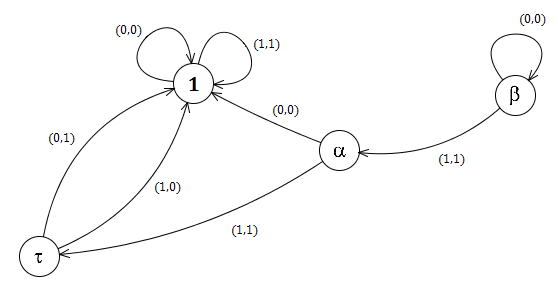
\includegraphics{groupAauto.png}
\end{center}


\noindent We then have that $\mathcal{A} = \langle \tau, \alpha, \beta \rangle$, where $\tau= (01)$, $\alpha = (1,\tau)$ and $\beta = (\beta, \alpha)$. \\ \\
We first observe that since $\alpha^{2} = 1$, that $\beta^{2} = (\beta^{2}, 1)$. Thus each of our generators has order 2. It follows now that $ \tau \alpha \tau \alpha = (\tau, \tau)$, and thus $(\tau \alpha)^{4} = 1$. We can also see that since $\alpha \beta = ( \beta, \tau \alpha)$, we have that $(\alpha \beta)^{4} = 1$. We also have that $\tau \beta \tau \beta = (\alpha \beta, \beta \alpha)$, and thus $(\tau \beta)^{8} = 1$. Thus, any subgroup created by two of the generators in $\mathcal{A}$ forms a quotient of one of the following dihedral groups: \\ \\
\centerline{$D_{4}(\tau, \alpha)$ $:=$ $\langle \tau, \alpha \rangle$ $=$ $\langle \tau, \alpha \mid \tau^{2} = \alpha^{2} = (\tau\alpha)^{4} = 1 \rangle$} \\
\centerline{$D_{8}(\tau, \beta)$ $:=$ $\langle \tau, \beta \rangle$ $=$ $\langle \tau, \beta \mid \tau^{2} = \beta^{2} = (\tau\beta)^{8} = 1 \rangle$} \\ 
\centerline{$D_{4}(\alpha, \beta)$ $:=$ $\langle \alpha, \beta \rangle$ $=$ $\langle \alpha, \beta \mid \alpha^{2} = \beta^{2} = (\alpha \beta)^{4} = 1 \rangle$} \\ \\
\noindent To represent any word $w$ in $\mathcal{A}$, we can write $w = (\tau) x_{1} \tau x_{2} \cdots \tau x_{n} (\tau) $, where $x_{i} \in D_{4}(\alpha, \beta)$. In order to write any word $w$ as an alternating word of $\tau$-letters and other generators, we can extend our generating set by making each of the elements in $D_{4}(\alpha, \beta)$ a new generator. If we do this, we should let the weight of each of these new generators just be the length according to the original generating set. This lets us not worry about having to find a minimal length representation of our word. We can then list out each of the unique elements that could go between $\tau$-letters: \\ \\
\begin{center}
\begin{tabular}{ c | c | c | c | c | c }
  name & element & pair & name & element & pair \\ \hline
  $\alpha_{1}$ & $\alpha$ & $(1, \tau)$ & $\beta_{1}$ & $\beta$ & $(\beta, \alpha)$\\ 
  $\alpha_{2}$ & $\alpha \beta$ & ($\beta, \tau \alpha)$ & $\beta_{2}$ & $\beta \alpha$ & $(\beta, \alpha \tau )$  \\ 
  $\alpha_{3}$ & $\alpha \beta \alpha$ & $(\beta, \tau \alpha \tau)$ & $\beta_{3}$ & $\beta \alpha \beta$ & $(1, \alpha \tau \alpha)$ \\ 
  $\alpha_{4}$ & $\alpha \beta \alpha \beta$ & $(1, \tau \alpha \tau \alpha)$ & \\ 
\end{tabular}
\end{center}
\vspace{10mm}
With this extended generating set in hand, we can set up a new definition: \\ \\
\begin{definition}
A word $(\tau) x_{1} \tau \cdots \tau x_{n} (\tau)$ is called a \textbf{reduced word} if each $x_{i}$ is equal to a non-$\tau$ letter in the extended generating set. A generator is then said to \textbf{occur} or be \textbf{contained} in $w$ if it appears as a subword of $w$.  A word is also said to be \textbf{reducible} if it is not a reduced word. \\ \\
\end{definition}
Our goal now will be to apply Proposition 3.3 to prove subexponential growth. Our first step then should be to choose weights for our generators. It is important to recognize that we need to find an appropriate weight system that will minimize the amount of words that get no reduction when we split them (minimally, we should never increase the length of the word). To do this, we should try and set up some parameters for our weights so they minimize the amount of words that do not get any reduction when split into pair notation. We can do this by looking at some examples: \\ \\
From $\tau \beta \tau \beta = (\alpha \beta, \beta \alpha)$, we need to have $\ell(\tau) \geq \ell(\alpha)$. This follows from the fact that the length of $\tau \beta \tau \beta$ is $2 \ell(\tau) + 2 \ell(\beta)$. The sum of the lengths of the words in the left and right coordinates of the pair notation is then $2 \ell(\alpha) + 2 \ell(\beta)$. We want to ensure that in the worst case scenario, we never increase the length of a word when we split it up. So as a minimal restriction, we need to have $2 \ell(\tau) + 2 \ell(\beta) \geq 2 \ell(\alpha) + 2 \ell(\beta)$. After cancellation, we then see that we at least need to satisfy $\ell(\tau) \geq \ell(\alpha)$.  \\ \\
In addition, $\tau \alpha \beta \alpha \tau \alpha \beta \alpha = (\tau \alpha \tau \beta, \beta \tau \alpha \tau)$, which forces us to have $\ell(\alpha) \geq \ell(\tau)$, and thus $\ell(\tau) = \ell(\alpha)$ from the first inequality. Lastly, if we look at $\tau \beta \alpha \beta \tau \beta \alpha \beta  = ( \alpha \tau \alpha, \alpha \tau \alpha) $, we have $ 2\ell(\beta) \geq \ell(\alpha)$. We now propose the weight system: \\ \\
$$\ell(\tau) = 1, \ell(\alpha) = 1, \ell(\beta) = 1 $$ \\ \\
It will not necessarily be the case that we can get all of our words to reduce in length when we split them. To prepare us for this case, we should try to at least have a global bound on the number of words of arbitrary length that get no reduction. Otherwise, it will be difficult to control the proportion of words that get less than a certain amount of reduction, a condition required to prove subexponential growth by Proposition 3.3. The following definitions will set our argument up so that we can find such a global bound. \\ \\
Let $w$ be a reduced word that contains an even number of $\tau$-letters. When we split $w$ into its pair notation, we will be looking for length reduction in two fundamental ways; we either create words in the pair notation that have a smaller length than $w$, or we create words in the pair notation that are reducible. \\  
\begin{definition}:
Let $w$ be a reduced word containing an even occurrence of $\tau$-letters. We define the \textbf{first-line production of $w$} to be the product of the following algorithm: \\ \\
\begin{enumerate} 
\item Take a reduced word $w = (\tau) x_{1} \tau \cdots \tau x_{n} (\tau)$ that has an even occurrence of $\tau$-letters and expand each $x_{i}$ into its pair notation, denoted by $(x_{{i}_L},x_{{i}_R})$. If $w$ represents an element in $D_{4}(\alpha, \beta)$, skip to $(3)$, otherwise go to $(2)$. \\ \\
\item Take the leftmost string of the form $\tau (x_{{i}_L},x_{{i}_R})$ inside $w$ and use the property $\tau (x_{{i}_L},x_{{i}_R})$ = $ (x_{{i}_R},x_{{i}_L}) \tau$ to re-write $\tau (x_{{i}_L},x_{{i}_R})$ as $(x_{{i}_R},x_{{i}_L}) \tau$. Since $w$ has an even occurrence of $\tau$-letters, every time we use this re-writing rule we get the cancellation of 2 $\tau$-letters. This can be seen as follows for a string inside a word $w$: \\ \\
$ \tau x_{i} \tau x_{i+1} = \tau (x_{{i}_L},x_{{i}_R}) \tau (x_{{i+1_L}},x_{{i+1}_R}) = (x_{{i}_R},x_{{i}_L}) \tau \tau (x_{{i+1_L}},x_{{i+1}_R}) = (x_{{i}_R},x_{{i}_L})(x_{{i+1_L}},x_{{i+1}_R}) $.\\ \\
We can then see that we can perform $(2)$ multiple times until there are no remaining $\tau$-letters. Assuming we have done so, we can then proceed to $(3)$. \\ \\
\item Now that we have a word that can be expressed as a product of elements each of which is represented in the pair notation, we can multiply the elements in the left coordinate together and multiply elements in the right coordinate together. We should not perform any potential cancellation or reduction that could happen after we multiply elements together. We then call this final product the \textbf{first-line production of w}, which we will denote by $FL_{P}(w)$. \\ \\
\end{enumerate}
\end{definition}
\noindent It will be necessary to find a subgroup of finite index in $\mathcal{A}$ to satisfy the conditions of Proposition 3.3. The simplest choice is to consider the stabilizer of the nth level of the tree, denoted by $\mathcal{A}_n$. A word representing an element in $\mathcal{A}_n$ must contain an even number of $\tau$-letters or else it acts directly on the first level of the tree (assuming $n \geq 1)$. Thus it suffices to restrict our attention to reduced words that contain an even occurrence of $\tau$-letters as we did above. \\ \\
\begin{definition}
Let $(\phi_{L}, \phi_{R}) \colon \mathcal{A}_1 \to \mathcal{A} \times \mathcal{A}$ be the injective homomorphism that takes an element $x$ containing an even number of $\tau$-letters and writes it as an ordered pair, where $\phi_{L}(x)$ and $\phi_{R}(x)$ are the left and right coordinates of the pair notation respectively. An element $x \in D_{4}(\alpha, \beta)$ is \textbf{good by nature} if the following condition holds: $\ell(\phi_{L}(x)) + \ell(\phi_{R}(x)) < \ell(\tau) + \ell(x)$. \\ \\ 
\end{definition} 
\noindent This definition allows us to identify the simplest cases of reduction we could have inside a word $w$, as just having the occurrence of a good by nature element guarantees some type of reduction after we split it. This follows from the fact that since a reduced word can be written as $(\tau) x_{1} \tau \cdots \tau x_{n} (\tau)$, except for a potential case at the beginning or end of a word, we can associate to each $x_{i}$ a $\tau$-letter. Then, since $\tau$ cannot be represented in pair notation, when we split the reduced word, we immediately lose the weight of one $\tau$-letter for each $x_{i}$. The exception mentioned above is ultimately not problematic, as that case can only occur in at most one place in any given word. \\ \\
We can now look at each of our non-$\tau$ generators then to see if they are good by nature: \\ \\
\begin{center}
\begin{tabular}{ c | c | c | c | c | c }
  $x$ & $\ell(\tau) + \ell(x)$ & $\ell(\phi_{L}(x)) + \ell(\phi_{R}(x))$ & $x$ & $\ell(\tau) + \ell(x)$ & $\ell(\phi_{L}(x)) + \ell(\phi_{R}(x))$ \\ \hline
  $\alpha_{1}$ & 2 & 1 & $\beta_{1}$ & 2 & 2\\ 
  $\alpha_{2}$ & 3 & 3 & $\beta_{2}$ & 3 & 3  \\ 
  $\alpha_{3}$ & 4 & 4 & $\beta_{3}$ & 4 & 3 \\ 
  $\alpha_{4}$ & 5 & 4 & \\ 
\end{tabular}
\end{center}
\vspace{10mm}
Our good by nature elements are thus: $\alpha_{1}$, $\alpha_{4}$, and $\beta_{3}$. We should now try and distinguish between elements that lead to reduction and those that do not.  \\ \\
\begin{definition}
\label{primitive}
A \textbf{primitive set $\mathcal{S}$ of good blocks} is a finite set of reduced words (the good blocks) that have an even occurrence of $\tau$-letters such that each $w \in \mathcal{S}$ satisfies one of the following: \\ \\
$(i)$ For $FL_{P}(w) = (w_{L},w_{R})$, at least one of $w_{L}$ or $w_{R}$ is reducible. \\ \\
$(ii)$ A good by nature element occurs between two $\tau$-letters in one of the reduced coordinates of $FL_{P}(w)$, and that coordinate is also in $\mathcal{A}_1$. \\ \\
$(iii)$ For $FL_{P}(w) = (w_{L}, w_{R})$, either $FL_{P}(w_{L})$ or $FL_{P}(w_{R})$ has a reduced coordinate in $\mathcal{A}_1$ that has an occurrence of a good by nature element in between two $\tau$ letters. \\ \\
$(iv)$ The element represented by $w$ is good by nature. \\ \\
$(v)$ For $FL_{P}(w_L) = (w_{LL}, w_{RR})$ and $FL_{P}(w_R) = (w_{RL},w_{RR})$, either $FL_{P}(w_{LL})$, $FL_{P}(w_{LR})$, $FL_{P}(w_{RL})$, or $FL_{P}(w_{RR})$  has a reduced coordinate that is in $\mathcal{A}_1$ and has an occurrence of a good by nature element in between two $\tau$ letters.
\end{definition}
\begin{definition}
An \textbf{$\mathcal{S}$-bad block} is a reduced word $(\tau) x_{1} \tau \cdots \tau x_{n} (\tau)$ containing no occurrence of any $w \in \mathcal{S}$. \\ \\
\end{definition}
\noindent Our goal will now be the following: \\ \\
$(*)$ Find an appropriate primitive set $\mathcal{S}$ of good blocks such that the number of $\mathcal{S}$-bad blocks containing $i$ non-$\tau$ letters is globally bounded by some $M$, for any $i$. \\ \\
\begin{proposition}
There is a primitive set $\mathcal{S}$ of good blocks for the subgroup $\mathcal{A}_3$ that satisfies $(*)$. \\ \\
\end{proposition}
\begin{proof}
We first propose the following primitive set $\mathcal{S}$ of good blocks: \\ \\
$\mathcal{S} = \Bigg(\displaystyle{ \bigcup_{i=1}^{8}P_{i}} \Bigg)\cup\{\alpha_{1} \}\cup \{\alpha_{4} \}\cup \{\beta_{3} \}\cup \{\alpha_{3} \}$, where each $P_{i}$ is defined below.\\ \\
It is easy to see that $\alpha_{1}$, $\alpha_{4}$, and $\beta_{3}$ satisfy condition $(iv)$ of Definition (\ref{primitive}) to be in a primitive set of good blocks. Since $FL_{P}(\alpha_{3}) = (\beta, \tau \alpha \tau)$, it follows that $\tau \alpha \tau$ contains an occurrence of a good by nature element isolated between two $\tau$-letters, so $\alpha_{3}$ satisfies condition $(ii)$ of Definition (\ref{primitive}). We will now define each $P_{i}$ and verify that each set consists of blocks that are in $\mathcal{S}$. \\ \\
First, observe that if we let $\Box$ be an arbitrary element in the set $\{ \beta_{1}, \beta_{2}, \alpha_{2} \}$ and $FL_{P}(\Box) = (\Box_{L}, \Box_{R})$, then $\Box_{L} = \beta$. It follows then that for $w = \tau \Box \tau$, we have $w_{R} = \beta$. \\ \\
From here define the following sets that contain blocks in $\mathcal{S}$. \\ \\  
\underline{$P_{1}$}: For a block $b \in P_{1}$, $b$ has the form $\tau \Box \tau \beta_{1} \tau \Box \tau \beta_{1} \tau \Box \tau$ and creates the string $\beta \alpha \beta \alpha \beta$ in $b_{R}$. Thus, every word in $P_{1}$ meets condition $(i)$ of Definition (\ref{primitive}) as $\beta \alpha \beta \alpha \beta$ can be reduced to $\alpha \beta \alpha$. \\ \\
\underline{$P_{2}$}: For a block $b \in P_{2}$, $b$ has the form $\Box^{*} \tau \Box \tau \beta_{1} \tau \Box \tau \beta_{2}$ and creates the string $\Box^{*}_{R} \beta \alpha \beta \alpha \tau$ in $b_{R}$. Since $\Box^{*}_{R}$ can only contain $\alpha$ or $\tau$-letters, it follows that if $\Box^{*}_{R}$ ends in $\tau$, we meet condition $(ii)$. If  $\Box^{*}_{R}$ ends in $\alpha$, then we meet condition $(i)$. Thus, every word in $P_{2}$ meets either condition $(i)$ or $(ii)$. \\ \\
\underline{$P_{3}$}: For a block $b \in P_{3}$, $b$ has the form  $ \beta_{2} \tau \Box \tau \beta_{1} \tau \Box \tau \alpha_{2}$ or $ \alpha_{2} \tau \Box \tau \beta_{1} \tau \Box \tau \alpha_{2}$ and creates $\alpha \tau \beta_{3} \tau \alpha$ or $\tau \alpha_{4} \tau \alpha$ respectively in $b_{R}$. Thus, in either case, every word in $P_{3}$ meets condition $(ii)$. \\ \\
\underline{$P_{4}$}: For a block $b \in P_{4}$, $b$ has the form  $\tau \Box \tau \beta_{1} \tau \Box \tau \beta_{1} \tau \Box \tau \alpha_{2}$ and creates $\beta \alpha \beta \alpha \beta \tau \alpha$ in $b_{R}$. Thus, every word in $P_{4}$ meets condition $(i)$. \\ \\
\underline{$P_{5}$}: For a block $b \in P_{5}$, $b$ has the form  $\beta_{2} \tau \Box \tau \beta_{1} \tau \Box \tau \beta_{2}$ and creates $\alpha \tau \alpha_{4} \tau$ in $b_{R}$. Thus, in either case, every word in $P_{5}$ meets condition $(ii)$. \\ \\
\underline{$P_{6}$}: For a block $b \in P_{6}$, $b$ has the form $\tau \Box \tau \beta_{2} \tau \Box \tau \beta_{2} \tau \Box \tau \alpha_{2} \tau \Box \tau \alpha_{2}$ and creates $\beta \alpha \tau \beta_{2} \tau \beta_{1} \tau \alpha_{2} \tau \alpha$ in $b_{R}$. It follows then that $FL_{P}(b_{R})$ creates $\alpha \tau \beta_{3} \tau$ in $b_{RR}$. Thus, every word in $P_{6}$ meets condition $(iii)$.  \\ \\
\underline{$P_{7}$}: For a block $b \in P_{7}$, $b$ has the form  $\alpha_{2} \tau \Box \tau \beta_{1} \tau \Box \tau \Box^{*}$ and creates $\tau \alpha \beta \alpha \beta \Box^{*}_{R}$ in $b_{R}$. Since $\Box^{*}_{R}$ can only contain $\alpha$ or $\tau$-letters, it follows that if $\Box^{*}_{R}$ begins with $\alpha$, then we satisfy condition $(i)$. If $\Box^{*}_{R}$ begins with $\tau$, then we satisfy condition $(ii)$. Thus, every word in $P_{7}$ satifies condition $(i)$ or $(ii)$. \\ \\
\underline{$P_{8}$}: For a block $b \in P_{8}$, $b$ has the form  $\alpha_{2} \tau \Box \tau \beta_{2}$ and creates $\tau \alpha_{3} \tau$ in $b_{R}$. It follows then that $b_{RL}$ contains $\tau \alpha_{1} \tau$. Thus, every word in $P_{8}$ meets condition $(iii)$. \\ \\ 
Now that we have our primitive set $\mathcal{S}$, we can prove the proposition. Since a reduced word $w$ is of the form $\cdots \tau x_{i-1} \tau x_{i} \tau x_{i+1} \cdots$, if $w$ is an $\mathcal{S}$-bad block, then it cannot contain an occurrence of $\alpha_{1}, \alpha_{3}, \alpha_{4}$, or $\beta_{3}$. Thus, every $\mathcal{S}$-bad block is of the form $\cdots \tau \Box \tau \Box \tau \cdots$ \\ \\
We can then show that the number of ways to arrange the elements from $ \{ \alpha_{2}, \beta_{1}, \beta_{2} \} $ in an $\mathcal{S}$-bad block is finite, and hence we have a global bound.  \\ \\
Consider an arbitrary $\mathcal{S}$-bad word of the form: $\cdots \tau \Box \tau \Box \tau \Box_{1} \tau \Box_{2} \tau \Box_{3} \tau \Box_{4} \tau \cdots $ It is sufficient to only show that there are a finite number of choices for $\Box_{1}, \Box_{3}, \Box_{5}, \ldots$, since we must have the exact same restriction for $\Box_{2}, \Box_{4}, \Box_{6}, \ldots$, and thus there are only a finite number of choices for the whole word to remain an $\mathcal{S}$-bad block. Before we do a case analysis though, we should remark that we are allowed to assume our $\mathcal{S}$-bad block has sufficiently many non-$\tau$ letters in its reduced word to give the patterns described below. Otherwise we can say we have a finite bound since we would have only a finite number of cases that do not meet this condition.  \\ \\
\begin{enumerate}
\item $\Box_{1} = \alpha_{2}$ \\
Given this, we cannot have $\Box_{3} = \beta_{2}$ or else we create a block in $P_{8}$. If $\Box_{3} = \beta_{1}$, then regardless of our choice for $\Box_{5}$, we will create a block from $P_{7}$. Thus the only way a string  $\alpha_{2} \tau \Box \tau \beta_{1}$ can occur is at the end of a word in order to remain an $\mathcal{S}$-bad block. Essentially then, except for a small amount of variation at the beginning and end of the word, if $\Box_{i} = \alpha_{2}$, then $\Box_{i+2}$, $\Box_{i+4}, \cdots$ must all be $\alpha_{2}$.  \\ \\
\item $\Box_{1} = \beta_{1}$ \\ 
Given this, if $\Box_{3} = \beta_{2}$, then assuming there is at least $\Box \tau \Box \tau$ to the left of $\Box_{1}$, this creates a block from $P_{2}$. If $\Box_{3} = \beta_{1}$, assuming there is at least $\tau \Box \tau$ to the left of $\Box_{1}$ and $\tau \Box \tau$ to the right of $\Box_{3}$, this creates a block from $P_{1}$.  If $\Box_{3} = \alpha_{2}$, then assuming there is at least $\tau \Box \tau \Box \tau \Box \tau$ to the left of $\Box_{1}$, we create a word from either $P_{3}$ or $P_{4}$. Thus, the only place $\beta_{1}$ can appear is near the beginning or end of a word, otherwise we make a good block from $\mathcal{S}$. \\ \\
\item $\Box_{1} = \beta_{2}$ \\
Given this, say $\Box_{3} = \beta_{1}$. If $\Box_{5} = \beta_{2}$, we create a block in $P_{5}$. If $\Box_{5} = \alpha_{2}$, then we create a block in $P_{3}$. If $\Box_{5}$ = $\beta_{1}$, then assuming we have at least $\tau \Box \tau$ to the right of $\Box_{5}$, we have made a block in $P_{1}$. Thus, $\beta_{2} \tau \Box \tau \beta_{1}$ can only appear near the beginning or end of a word. Say now that $\Box_{3} = \alpha_{2}$, then as a result from case $(1)$, $\Box_{5}, \Box_{7}, \cdots$ must all be $\alpha_{2}$, except for some variation at the end of the word. \\ \\
\end{enumerate}
We discovered in case $(1)$ that if $\alpha_{2}$ occurs in an $\mathcal{S}$-bad block at position $i$ in a word $w$ then every letter at position congruent to $i$ modulo 4 to the right of $i$ must also be $\alpha_{2}$. If $\beta_{2}$ occurs in a $\mathcal{S}$-bad block at position $i$ then we have 2 subcases to consider. \\ \\
The first subcase is we have a string of $\beta_{2}$-letters at positions $i$ modulo 4 up until position $j$, where $\alpha_{2}$ is at position $j$. Thus at every subsequent position $j$ modulo 4 we have $\alpha_{2}$. Every sufficiently long string of this form contains as a substring a block in $P_{6}$. Hence this subcase cannot occur in an $\mathcal{S}$-bad block. The other subcase to consider is that if we have $\beta_{2}$ at position $i$, then at every subsequent position $i$ modulo 4, we must also have $\beta_{2}$. This subcase then never creates a substring in $P_{i}$, for arbitrary $i$.  \\ \\
Thus if we fix either $\alpha_{2}$ or $\beta_{2}$ at position $i$ in a word, for sufficiently long words we can guarantee that every position $i$ modulo 4 to the right of $i$ must be the same letter that occurs at position $i$ except for some variation at the end of the word. \\ \\
It follows then that there is a global bound $M$ on the number of $\mathcal{S}$-bad blocks that contain $i$ non-$\tau$ letters since after we pick the first few non-$\tau$ letters at the end and beginning of a word, the rest of the word is essentially a proper power of one of the following words: $\beta_{2} \tau$, $\beta_{2} \tau \alpha_{2} \tau$, or $\alpha_{2} \tau$. 
\end{proof}
\noindent Let $\mathcal{A}_3$ be the subgroup in $\mathcal{A}$ that stabilizes the first three levels of the tree. Consider now the injective homomorphism $\phi \colon \mathcal{A}_3 \to \mathcal{A}^{8}$ that maps $g \in \mathcal{A}_3$ to the ordered 8-tuple \\ $(\phi_{LLL}(g), \phi_{LLR}(g), \cdots, \phi_{RRR}(g))$. \\ \\
We will now want to count the number of alternating words that represent elements in $\mathcal{A}_3$ that contain a certain proportion of good letters. First, fix some small $\epsilon > 0$. 
\begin{definition}
An alternating word $w$ containing $n$ non-$\tau$ letters is called \textbf{$\epsilon-$bad} if at most $\epsilon n$ of its non-$\tau$ letters occur in good blocks in $\mathcal{S}$. 
\end{definition}
\begin{definition}
A non-$\tau$ letter is called \textbf{good by position} if it belongs to a block in $\mathcal{S}$.
\end{definition}
We now propose the following bound on the number of $\epsilon$-bad elements in $\mathcal{A}_3$ containing $n$ non-$\tau$ letters, which we will denote by $b_{\epsilon}(n)$: \\ 
$$b_{\epsilon}(n) \leq 2 \displaystyle{ n \choose \lfloor \epsilon n \rfloor } 7^{ \lfloor \epsilon n \rfloor } M^{1 + \lfloor \epsilon n \rfloor} $$ \\ 
\begin{itemize}
\item The 2 accounts for the choice of starting with a $\tau$-letter or not. \\ 
\item The $\displaystyle{ n \choose \lfloor \epsilon n \rfloor }$ accounts for the number of ways to ways to designate positions for good by position letters. \\
\item The $7^{ \lfloor \epsilon n \rfloor }$ accounts for the maximium number of ways to place good by position letters. \\ 
\item The $M^{1 + \lfloor \epsilon n \rfloor}$ accounts for the maximum number of choices to place $\mathcal{S}$-bad blocks. The $1 + \lfloor \epsilon n \rfloor$ is explained by the fact that once we place our good by position letters, we break up the word into at most $1 + \lfloor \epsilon n \rfloor$ compartments to place $\mathcal{S}$-bad blocks. \\
\end{itemize}
Since all elements in the original generating set have equal length, a  word of length $r$ containing the most non-$\tau$ letters would begin and end with a non-$\tau$ letter. We thus have that any word of length $r$ contains at most $(r+1)/2$ non-$\tau$ letters. Denote by $ B_{\epsilon}(r)$ the number of words in $ \{g \in \mathcal{A}_3 \mid \ell(g) \leq r\} $ that contain at most $ \epsilon n $ non-$\tau$ letters. We then have the following inequality: \\ \\ $$ B_{\epsilon}(r) \leq \displaystyle{ \sum_{n=0}^{(r+1)/2} b_{\epsilon}(n) } \leq \displaystyle{  (r+1) \displaystyle{ (r+1)/2 \choose \lfloor \epsilon (r+1)/2 \rfloor } 7^{ \lfloor \epsilon (r+1)/2 \rfloor } M^{1 + \lfloor \epsilon (r+1)/2 \rfloor} } $$. \\ \\
\begin{proposition}
$\mathcal{A}$ has subexponential growth.
\end{proposition}
\begin{proof}
Assume now that $\mathcal{A}$ has exponential growth. Then $\mathcal{A}_3$ has exponential growth as well \cite{BuxP}. Let $ \lambda > 1 $ be the growth rate of $\mathcal{A}_3$. By Stirling's formula, choose $\epsilon > 0$ so that $\lambda^{r}$ grows faster than the number of elements in $B_{\epsilon}(r)$.
We then observe then that for any $g \in \mathcal{A}_3$ represented by a word $w$ that contains a subword $v \in \mathcal{S}$, after splitting $w$ at most two times, we either create a reducible word or create a good by nature element between two $\tau$ letters. Thus, after splitting $w$ at most three times we are guaranteed to have reduction by at least some fixed amount. This is true since we either get immediate reduction in the former case, or get reduction after splitting again in the latter case. Since $\mathcal{S}$ is a finite set, there is a word that gets the worst reduction such that we can guarantee any other word in $\mathcal{S}$ reduces by at least that much.  Thus there is a number $\eta$ depending on $\epsilon$ that satisifies Proposition 3.3. This in turn implies that $\mathcal{A}_3$ has subexponential growth. 
\end{proof}
\begin{proposition}
$\mathcal{A}$ has superpolynomial growth. 
\end{proposition}
\begin{proof}
Consider $\mathcal{A}_1 \unlhd \mathcal{A}$ and let $ \phi \colon \mathcal{A}_1 \to \mathcal{A} \times \mathcal{A}$ be the injective homomorphism used before. It follows then that $\mathcal{A}_1 \cong \phi(\mathcal{A}_1)$. Let $N_{\tau}$ be the normal closure of $\tau$. It follows that the factor group $\mathcal{A}/N_{\tau}$ has order at most $ |\langle \alpha, \beta \rangle| = 8 $ since the coset $ \tau N_{\tau} = N_{\tau}$ in $ \mathcal{A}/N_{\tau} $.Thus $ [ \mathcal{A} \colon N_{\tau} ] \leq 8 $. \\ \\ Since $\alpha$ and $ \tau \alpha \tau $ are in $\mathcal{A}_1$, it follows that $\langle \phi(\alpha), \phi( \tau \alpha \tau ) \rangle$ $=$ $\langle (1, \tau), (\tau, 1) \rangle$  $\leq$ $\phi(\mathcal{A}_1)$. It is easy to see that $ N_{\tau} \times 1 \subset \phi(\mathcal{A}_1)$ since given any $x \in \mathcal{A}_1$ such that $\phi(x) = (x_{0},x_{1})$, we have that $\phi(x \tau \alpha \tau x^{-1}) = (x_{0}\tau x^{-1}_{0}, 1)$. Thus, by definition, the left coordinate of $\phi(x)$ is in $N_{\tau}$. Similarly, $1 \times N_{\tau} \subset \phi(\mathcal{A}_1)$, and thus $N_{\tau} \times N_{\tau} \subset \phi(\mathcal{A}_1)$.  \\ \\
Then $[\mathcal{A} \times \mathcal{A} : \phi(\mathcal{A}_1)] \leq [\mathcal{A} \times \mathcal{A} : N_\tau \times N_\tau] = [\mathcal{A} : N_\tau]^2 \leq 8^2 = 64$. This conclusion proves that $\mathcal{A}$ and $\mathcal{A} \times \mathcal{A}$ are commensurable. Using a known theorem \cite{Terp}, if a finitely generated infinite group $G$ is commensurable with $G^m$ then $G$ cannot have polynomial growth. Thus, $\mathcal{A}$ has super-polynomial growth. 
\end{proof}
\newpage
\subsection{Growth of $\mathcal{B}$}
Consider another quadratic polynomial $z^2 + c$ where $c$ is a root of $z^{16} + 8z^{15} + 28z^{14} +60z^{13} + 94z^{12} + 116z^{11} + 114z^{10} + 94z^{9} + 69z^{8} + 44z^{7} + 26z^{6} +14z^{5} + 5z^{4} + 2z^{3}$ such that the iterated monodromy group of this quadratic polynomial can be represented by the following automaton:
\centerline{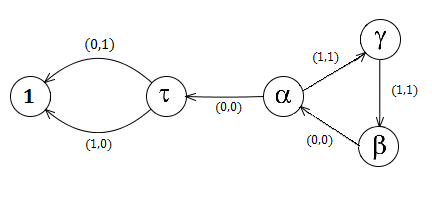
\includegraphics{groupBauto.png}}
We then have $\mathcal{B} = \langle \tau, \alpha, \beta, \gamma \rangle$, where $\tau= (01)$, $\alpha = (\tau,\gamma)$, $\beta = (\alpha, 1)$, and $\gamma = (1, \beta)$. \\ \\
We first observe that $\alpha^{2} = (\tau^{2}, \gamma^{2}) = (1, \gamma^{2})$. Thus, since $\beta^{2} = (\alpha^{2}, 1)$ and $\gamma^{2} = (1, \beta^{2})$, we have that $\alpha^{2} = \beta^{2} = \gamma^{2} = 1$. We first observe that $\tau \gamma \tau \gamma = (\beta, \beta)$, and thus $ (\tau \gamma)^{4} = 1$. From here we can see that since $\tau \alpha \tau \alpha = (\gamma \tau, \tau \gamma)$, we must have $(\tau \alpha)^{8} = 1$.  It now follows that $ \alpha \beta = ( \tau \alpha, \gamma)$ must have order 8 as well. We can also see that $ \beta \gamma = ( \alpha, \beta)$ has order 2, and so $\alpha \gamma = (\tau, \gamma \beta)$ must have order 2 as well. Lastly, we can see that $\tau \beta \tau \beta = (\alpha, \alpha)$, and thus $(\tau \beta)^{4} = 1$. We thus have that have any two of the generators in $\mathcal{B}$ forms a quotient of one of the following dihedral groups: \\ \\
\centerline{$D_{8}(\tau, \alpha)$ $:=$ $\langle \tau, \alpha \rangle$ $=$ $\langle \tau, \alpha \mid \tau^{2} = \alpha^{2} = (\tau\alpha)^{8} = 1 \rangle$} \\
\centerline{$D_{4}(\tau, \beta)$ $:=$ $\langle \tau, \beta \rangle$ $=$ $\langle \tau, \beta \mid \tau^{2} = \beta^{2} = (\tau\beta)^{4} = 1 \rangle$} \\ 
\centerline{$D_{4}(\tau, \gamma)$ $:=$ $\langle\tau, \gamma \rangle$ $=$ $\langle \tau, \gamma \mid \tau^{2} = \gamma^{2} = (\tau\gamma)^{4} = 1 \rangle$} \\ 
\centerline{$D_{8}(\alpha, \beta)$ $:=$ $\langle \alpha, \beta \rangle$ $=$ $\langle \alpha, \beta \mid \alpha^{2} = \beta^{2} = (\alpha \beta)^{8} = 1 \rangle$} \\ 
\centerline{$D_{2}(\alpha, \gamma)$ $:=$ $\langle \alpha, \gamma \rangle$ $=$ $\langle \alpha, \gamma \mid \alpha^{2} = \gamma^{2} = (\alpha \gamma)^{2} = 1 \rangle$} \\ 
\centerline{$D_{2}(\beta, \gamma)$ $:=$ $\langle \beta, \gamma \rangle$ $=$ $\langle \beta, \gamma \mid \beta^{2} = \gamma^{2} = (\beta \gamma)^{2} = 1 \rangle$} \\ \\
Since we want to represent any word $w$ in $\mathcal{B}$ as $w = (\tau) x_{1} \tau x_{2} \cdots \tau x_{n} (\tau) $, where $x_{i} \in \langle \alpha, \beta, \gamma \rangle$, we should first verify that $\langle \alpha, \beta, \gamma \rangle$ has finite order. \\ \\
Using the homomorphism $\phi$ from the previous section, we can see that given any $x \in \langle \alpha, \beta, \gamma \rangle$, we have that $\phi_{L}(x) \subset D_{8}(\tau, \alpha)$ which has order 16 and $\phi_{R}(x) \subset D_{2}(\beta, \gamma)$ which has order 4. It follows then that $ \left| \langle \alpha, \beta, \gamma \rangle \right| \leq 64$. Consider now the coset space $ \langle \alpha, \beta, \gamma \rangle  / D_{8} (\alpha, \beta )$. We first realize that since $\alpha \gamma = \gamma \alpha$ and $\beta \gamma = \gamma \beta$, any $x \in \langle \alpha, \beta, \gamma \rangle$ contains at most one $\gamma$ or else we can move $\gamma$-letters through $x$ until we get cancellation. Observing that $\gamma$ commutes with $\alpha$ and $\beta$, we can then write any $x \in \langle \alpha, \beta, \gamma \rangle$ that contains one $\gamma$-letter as $x = \gamma y$, where $y \in D_{8}(\alpha, \beta)$. If we then consider the coset $x D_{8}(\alpha, \beta)$, we have $x D_{8}(\alpha, \beta) = \gamma y D_{8} ( \alpha \beta ) = \gamma D_{8} (\alpha, \beta)$. It follows that $[ \langle \alpha, \beta, \gamma \rangle \colon D_{8}(\alpha, \beta) ]$ = 2, and hence $D_{8}(\alpha, \beta) \unlhd \langle \alpha, \beta, \gamma \rangle$. We then have that $|\langle \alpha, \beta, \gamma \rangle| = 2 \cdot |D_{8}(\alpha, \beta)| = 2 \cdot 16 = 32$. \\ \\
We will again want to write any word $w$ as an alternating word of $\tau$-letters and other generators, so we can extend our generating set by making each of the elements in $\langle \alpha, \beta, \gamma \rangle$ a new generator: 
\newpage
\centerline{
\begin{tabular}{ c | c | c | c | c | c}
  name & element & pair & name & element & pair \\ \hline
  $s_{1}$ & $\gamma$ & $(1, \beta)$ &   $s_{17}$ & $\beta \alpha \beta \alpha \beta \alpha \beta$ & $(\alpha \tau \alpha \tau \alpha \tau \alpha, \gamma)$  \\ 
  $s_{2}$ & $\beta$ & $(\alpha, 1)$ & $s_{18}$ & $\gamma \alpha$ & $(\tau, \beta \gamma)$ \\ 
  $s_{3}$ & $\gamma \beta$ & $(\alpha, \beta)$ & $s_{19}$ & $ \gamma \alpha \beta$ & $(\tau \alpha, \beta \gamma)$  \\ 
  $s_{4}$ & $\alpha$ & $(\tau, \gamma)$ & $s_{20}$ & $\gamma \alpha \beta \alpha$ & $(\tau \alpha \tau, \beta)$  \\ 
  $s_{5}$ & $\alpha \beta$ & $(\tau \alpha, \gamma)$ & $s_{21}$ & $\gamma \alpha \beta \alpha \beta$ & $(\tau \alpha \tau \alpha, \beta)$ \\ 
  $s_{6}$ & $\alpha \beta \alpha$ & $(\tau \alpha \tau, 1)$ & $s_{22}$ & $\gamma \alpha \beta \alpha \beta \alpha$ & $(\tau \alpha \tau \alpha \tau, \beta \gamma)$ \\ 
  $s_{7}$ & $\alpha \beta \alpha \beta$ & $(\tau \alpha \tau \alpha, 1)$ & $s_{23}$ & $\gamma \alpha \beta \alpha \beta \alpha \beta$ & $(\tau \alpha \tau \alpha \tau \alpha, \beta \gamma)$ \\ 
  $s_{8}$ & $\alpha \beta \alpha \beta \alpha$ & $(\tau \alpha \tau \alpha \tau, \gamma)$ & $s_{24}$ & $\gamma \alpha \beta \alpha \beta \alpha \beta \alpha$ & $(\tau \alpha \tau \alpha \tau \alpha \tau, \beta)$  \\
  $s_{9}$ & $\alpha \beta \alpha \beta \alpha \beta$ & $(\tau \alpha \tau \alpha \tau \alpha, \gamma)$ & $s_{25}$ & $\gamma \alpha \beta \alpha \beta \alpha \beta \alpha \beta$ & $(\tau \alpha \tau \alpha \tau \alpha \tau \alpha, \beta)$  \\ 
  $s_{10}$ & $\alpha \beta \alpha \beta \alpha \beta \alpha$ & $(\tau \alpha \tau \alpha \tau \alpha \tau, 1)$ & $s_{26}$ & $\gamma \beta \alpha$ & $(\alpha \tau, \beta \gamma)$ \\
  $s_{11}$ & $\alpha \beta \alpha \beta \alpha \beta \alpha \beta$ & $(\tau \alpha \tau \alpha \tau \alpha \tau \alpha, 1)$ & $s_{27}$ &  $\gamma \beta \alpha \beta$ & $(\alpha \tau \alpha, \beta \gamma)$ \\
  $s_{12}$ & $\beta \alpha$ & $(\alpha \tau, \gamma)$ & $s_{28}$ & $\gamma \beta \alpha \beta \alpha$ & $(\alpha \tau \alpha \tau, \beta)$  \\
  $s_{13}$ & $\beta \alpha \beta$ & $(\alpha \tau \alpha, \gamma)$ & $s_{29}$ & $\gamma \beta \alpha \beta \alpha \beta$ & $(\alpha \tau \alpha \tau \alpha, \beta)$ \\
  $s_{14}$ & $\beta \alpha \beta \alpha$ & $(\alpha \tau \alpha \tau, 1)$ & $s_{30}$ &  $\gamma \beta \alpha \beta \alpha \beta \alpha$ & $(\alpha \tau \alpha \tau \alpha \tau, \beta \gamma)$  \\
  $s_{15}$ & $\beta \alpha \beta \alpha \beta$ & $(\alpha \tau \alpha \tau \alpha, 1)$ & $s_{31}$ & $\gamma \beta \alpha \beta \alpha \beta \alpha \beta$ & $(\alpha \tau \alpha \tau \alpha \tau \alpha, \beta \gamma)$ \\
  $s_{16}$ & $\beta \alpha \beta \alpha \beta \alpha$ & $(\alpha \tau \alpha \tau \alpha \tau, \gamma)$ \\
 \\   
\end{tabular}
}
\vspace{5mm}
\noindent We should again determine what types of restrictions we can have on our lengths: \\ 
\hspace*{50 mm}$\tau \alpha \tau \alpha = (\gamma \tau, \tau \gamma) \Rightarrow \ell(\alpha) \geq \ell(\gamma)$. \\
\hspace*{50 mm}$\tau \alpha \beta \tau \alpha \beta = ( \gamma \tau \alpha, \tau \alpha \gamma) \Rightarrow \ell(\beta) \geq \ell(\gamma)$. \\
\hspace*{50 mm}$ \tau \gamma \alpha \tau \gamma \alpha = (\beta \gamma \tau, \tau \beta \gamma) \Rightarrow \ell(\alpha) \geq \ell(\beta)$. \\
\hspace*{50 mm}$ \tau \gamma \beta \alpha \beta \tau \gamma \beta \alpha \beta = (\gamma \beta \alpha \tau \alpha, \alpha \tau \alpha \tau \gamma \beta) \Rightarrow \ell(\beta) \geq \ell(\alpha)$. \\ \\
\noindent From the last two inequalities that we must have $\ell(\alpha) = \ell(\beta)$. We now propose the weight system: \\ \\ 
\centerline{$\ell(\tau) = 3, \ell(\gamma) = 6, \ell(\alpha) = 7, \ell(\beta) = 7$} \\ \\
\noindent We can look at each of our non-$\tau$ letters then to see which elements are good by nature: \\ \\
\centerline{\begin{tabular}{ c | c | c | c | c | c}
  $x$ & $\ell(\tau) + \ell(x)$ & $\ell(\phi_{L}(x)) + \ell(\phi_{R}(x))$ & $x$ & $\ell(\tau) + \ell(x)$ & $\ell(\phi_{L}(x)) + \ell(\phi_{R}(x))$ \\ \hline
  $s_{1}$ & 9 & 7 & $s_{17}$ & 52 & 43\\ 
  $s_{2}$ & 10 & 7 & $s_{18}$ & 16 & 16\\ 
  $s_{3}$ & 16 & 14 & $s_{19}$ & 23 & 23\\ 
  $s_{4}$ & 10 & 9 & $s_{20}$ & 30 & 20\\ 
  $s_{5}$ & 17 & 16 & $s_{21}$ & 37 & 27\\ 
  $s_{6}$ & 24 & 13 & $s_{22}$ & 44 & 36\\ 
  $s_{7}$ & 31 & 20 & $s_{23}$ & 51 & 43\\ 
  $s_{8}$ & 38 & 29 & $s_{24}$ & 58 & 40\\ 
  $s_{9}$ & 45 & 36 & $s_{25}$ & 65 & 47\\ 
  $s_{10}$ & 52 & 33 & $s_{26}$ & 23 & 23\\ 
  $s_{11}$ & 59 & 40 & $s_{27}$ & 30 & 30\\ 
  $s_{12}$ & 17 & 16 & $s_{28}$ & 37 & 27\\ 
  $s_{13}$ & 24 & 23 & $s_{29}$ & 44 & 34\\ 
  $s_{14}$ & 31 & 20 & $s_{30}$ & 51 & 43\\ 
  $s_{15}$ & 38 & 27 & $s_{31}$ & 58 & 50\\ 
  $s_{16}$ & 45 & 36 \\ 
\end{tabular} }
\newpage
\noindent Denote by $\mathcal{G}$ the set of good by nature elements. It follows then that the only non-$\tau$ generators not in $\mathcal{G}$ are $s_{18}$, $s_{19}$, $s_{26}$, and $s_{27}$. Let $\Box$ denote any of the elements in $\{ s_{18}, s_{19}, s_{26}, s_{27}  \}$, and we notice that for $FL_{P}(\Box) = (\Box_{L}, \Box_{R} )$, we have that $\Box_{R} = \beta \gamma$. \\ \\

\begin{proposition}
There is a primitive set $\mathcal{S}$ of good blocks for the subgroup $\mathcal{B}_4$ that satisfies $(*)$. \\ \\
\end{proposition}
\begin{proof}
We first propose the primitive set $\mathcal{S} = \Bigg(\displaystyle{ \bigcup_{i=1}^{12}P_{i}} \Bigg) \cup \mathcal{G}$, where each $P_{i}$ is defined below. \\ \\
It is easily seen that every element of $\mathcal{G}$ satisfies condition $(iv)$ of Definition (\ref{primitive}) to be in a primitive set of good blocks. \\ \\
\underline{$P_{1}$}: For a block $b \in P_{1}$, $b$ has the form $s_{18} \tau \Box \tau s_{18}$ and creates the string $\tau s_{3} \tau$ in $b_{L}$. Thus, every word in $P_{1}$ meets condition $(ii)$ of Definition (\ref{primitive}). \\ \\
\underline{$P_{2}$}: For a block $b \in P_{2}$, $b$ has the form $s_{18} \tau \Box \tau s_{19}$ and creates the string $\tau s_{3} \tau \alpha$ in $b_{L}$. Thus, every word in $P_{2}$ meets condition $(ii)$. \\ \\
\underline{$P_{3}$}: For a block $b \in P_{3}$, $b$ has the form $\tau \Box \tau s_{18} \tau \Box \tau s_{26} \tau \Box \tau$ and creates the string $\beta \gamma \tau s_{26} \tau \beta \gamma$ in $b_{L}$. It follows then that $FL_{P}(b_{L})$ creates the string $\alpha \beta \gamma \alpha$ in $b_{LL}$, and $FL_{P}(b_{LL})$ creates the string $\tau s_{4} \tau$ in $b_{LLL}$.  Thus, every word in $P_{3}$ meets condition $(v)$. \\ \\
\underline{$P_{4}$}: For a block $b \in P_{4}$, $b$ has the form $\tau \Box \tau s_{19} \tau \Box \tau s_{18} \tau \Box \tau$ and creates the string $\beta \gamma \tau s_{19} \tau \beta \gamma$ in $b_{L}$. It follows then that $FL_{P}(b_{L})$ creates the string $\alpha \beta \gamma \alpha$ in $b_{LL}$, and $FL_{P}(b_{LL})$ creates the string $\tau s_{4} \tau$ in $b_{LLL}$.  Thus, every word in $P_{4}$ meets condition $(v)$. \\ \\
\underline{$P_{5}$}: For a block $b \in P_{5}$, $b$ has the form $s_{19} \tau \Box \tau s_{26}$ and creates the string $\tau s_{20} \tau$ in $b_{L}$. Thus, every word in $P_{5}$ meets condition $(ii)$. \\ \\
\underline{$P_{6}$}: For a block $b \in P_{6}$, $b$ has the form $s_{19} \tau \Box \tau s_{27}$ and creates the string $\tau s_{20} \tau \alpha$ in $b_{L}$. Thus, every word in $P_{6}$ meets condition $(ii)$. \\ \\
\underline{$P_{7}$}: For a block $b \in P_{7}$, $b$ has the form $s_{26} \tau \Box \tau s_{18}$ and creates the string $\alpha \tau s_{3} \tau$ in $b_{L}$. Thus, every word in $P_{7}$ meets condition $(ii)$. \\ \\
\underline{$P_{8}$}: For a block $b \in P_{8}$, $b$ has the form $s_{26} \tau \Box \tau s_{19}$ and creates the string $\alpha \tau s_{3} \tau \alpha$ in $b_{L}$. Thus, every word in $P_{8}$ meets condition $(ii)$. \\ \\
\underline{$P_{9}$}: For a block $b \in P_{9}$, $b$ has the form $s_{26} \tau \Box \tau s_{27}$ and creates the string $\alpha \tau s_{26} \tau \alpha$ in $b_{L}$. It follows then that $FL_{P}(b_{L})$ creates $\tau s_{3} \tau$ in $b_{LL}$. Thus, every word in $P_{9}$ meets condition $(iii)$. \\ \\
\underline{$P_{10}$}: For a block $b \in P_{10}$, $b$ has the form $s_{27} \tau \Box \tau s_{19}$ and creates the string $\alpha \tau s_{19} \tau \alpha$ in $b_{L}$. It follows then that $FL_{P}(b_{L})$ creates $\tau s_{3} \tau$ in $b_{LL}$. Thus, every word in $P_{10}$ meets condition $(iii)$. \\ \\
\underline{$P_{11}$}: For a block $b \in P_{11}$, $b$ has the form $s_{27} \tau \Box \tau s_{26}$ and creates the string $\alpha \tau s_{20} \tau$ in $b_{L}$. Thus, every word in $P_{11}$ meets condition $(ii)$. \\ \\
\underline{$P_{12}$}: For a block $b \in P_{12}$, $b$ has the form $s_{27} \tau \Box \tau s_{27}$ and creates the string $\alpha \tau s_{20} \tau \alpha$ in $b_{L}$. Thus, every word in $P_{12}$ meets condition $(ii)$. \\ \\
Now that we have our primitive set $\mathcal{S}$, we can prove the proposition. Since a reduced word $w$ is of the form $\cdots \tau x_{i-1} \tau x_{i} \tau x_{i+1} \cdots$, if $w$ is an $\mathcal{S}$-bad block, then it cannot contain an occurrence of any element in $\mathcal{G}$. Thus, every $\mathcal{S}$-bad block is of the form $\cdots \tau \Box \tau \Box \tau \cdots$, where $\Box \in \{ s_{18}, s_{19}, s_{26}, s_{27} \}$. Once again if we can then show that the number of ways to arrange the elements from $\{ s_{18}, s_{19}, s_{26}, s_{27} \}$ in an $\mathcal{S}$-bad block is finite, we will have the global bound.  \\ \\
Consider an arbitrary $\mathcal{S}$-bad word of the form: $\cdots \tau \Box \tau \Box \tau \Box_{1} \tau \Box_{2} \tau \Box_{3} \tau \Box_{4} \tau \cdots $ It is sufficient to only show that there are a finite number of choices for $\Box_{1}, \Box_{3}, \Box_{5}, \ldots$, since we must have the exact same restriction for $\Box_{2}, \Box_{4}, \Box_{6}, \ldots$, and thus there are only a finite number of choices for the whole word to remain an $\mathcal{S}$-bad block. Before we do a case analysis though, we should once again assume our $\mathcal{S}$-bad block has sufficiently many non-$\tau$ letters to give the patterns described below. \\ \\
\begin{enumerate}
\item: $\Box_{1} = s_{18}$. \\ 
If $\Box_{3} = s_{18}$ or $s_{19}$, then we create either a block in either $P_{1}$ or $P_{2}$. If $\Box_{3} = s_{26}$, then assuming we have a $\tau \Box \tau$ before $\Box_{1}$ and after $\Box_{3}$, we create a block in $P_{3}$. Thus, if $\Box_{1} = s_{18}$, for sufficiently long words the only option to remain an $\mathcal{S}$-bad block is to have $\Box_{3} = s_{27}$. \\ \\
\item: $\Box_{1} = s_{19}$. \\
If $\Box_{3} = s_{18}$, then assuming we have a $\tau \Box \tau$ before $\Box_{1}$ and after $\Box_{3}$, we create a block in $P_{4}$. If $\Box_{3} = s_{26}$ or $s_{27}$, we create a block in either $P_{5}$ or $P_{6}$.  Thus, if $\Box_{1} = s_{18}$, for sufficiently long words the only option to remain an $\mathcal{S}$-bad block is to have $\Box_{3} = s_{19}$. \\ \\
\item: $\Box_{1} = s_{26}$. \\
If $\Box_{3} = s_{18}$, $s_{19}$, or $s_{27}$ then we create a block in either $P_{7}$, $P_{8}$, or $P_{9}$. Thus, if $\Box_{1} = s_{26}$, for sufficiently long words the only option to remain an $\mathcal{S}$-bad block is to have $\Box_{3} = s_{26}$. \\ \\
\item: $\Box_{1} = s_{27}$. \\
If $\Box_{3} = s_{19}$, $s_{26}$, or $s_{27}$ then we create a block in either $P_{10}$, $P_{11}$, or $P_{12}$. Thus, if $\Box_{1} = s_{27}$, for sufficiently long words the only option to remain an $\mathcal{S}$-bad block is to have $\Box_{3} = s_{18}$. \\ \\
\end{enumerate} 
Consider an arbitrary $\mathcal{S}$-bad block, call it $w$. Fix now the element $s_{19}$ at position $i$ in $w$. It follows then that every position $i$ modulo 4 must also feature $s_{19}$. If we fix $s_{26}$ at position $i$ in $w$, then every position $i$ modulo 4 must also feature $s_{26}$. If $w$ features $s_{18}$ at position $i$, then position $i$ modulo 8 must also feature $s_{18}$, and position $i + 4$ modulo 8 must feature $s_{27}$. We thus have the desired global bound $M$, since besides a finite amount of variation at the beginnings and ends of the word, every $\mathcal{S}$-bad block is essentially a proper power of one of the following words: $s_{18} \tau s_{19} \tau s_{27} \tau s_{19} \tau$, $s_{18} \tau s_{26} \tau s_{27} \tau s_{26} \tau$, $s_{18} \tau s_{18} \tau s_{27} \tau s_{27} \tau$, $s_{19} \tau$, $s_{19} \tau s_{27} \tau$, or $s_{27} \tau$. \\ \\
\end{proof}

\noindent Let $\mathcal{B}_4$ be the subgroup in $\mathcal{B}$ that stabilizes the first four levels of the tree. Consider now the injective homomorphism: \\ \\
$ \phi \colon \mathcal{B}_4 \to \mathcal{B}^{16}$ that maps $g \in \mathcal{B}_4$ to the ordered 16-tuple $(\phi_{LLLL}(g), \phi_{LLLR}(g), \cdots, \phi_{RRRR}(g))$. \\ \\
We now propose the following bound on the number of $\epsilon$-bad elements in $\mathcal{B}_4$ containing $n$ non-$\tau$ letters, which we will denote by $b_{\epsilon}(n)$: \\
$$b_{\epsilon}(n) \leq 2 \displaystyle{ n \choose \lfloor \epsilon n \rfloor } 31^{ \lfloor \epsilon n \rfloor } M^{1 + \lfloor \epsilon n \rfloor} $$ \\
\begin{itemize}
\item The 2 accounts for the choice of starting with a $\tau$-letter or not. \\
\item The $\displaystyle{ n \choose \lfloor \epsilon n \rfloor }$ accounts for the number of ways to ways to designate positions for good by position letters. \\
\item The $31^{ \lfloor \epsilon n \rfloor }$ accounts for the maximium number of ways to place good by position letters. \\
\item The $M^{1 + \lfloor \epsilon n \rfloor}$ accounts for the maximum number of choices to place $\mathcal{S}$-bad blocks. The $1 + \lfloor \epsilon n \rfloor$ is explained by the fact that once we place our good by position letters, we break up the word into at most $1 + \lfloor \epsilon n \rfloor$ compartments to place $\mathcal{S}$-bad blocks. \\
\end{itemize}

Since $\gamma$ is the lowest weight non-$\tau$ generator, a word of length $r$ containing the most non-$\tau$ letters would alternate between $\gamma$-letters and $\tau$-letters. We thus have that any word of length $r$ contains at most $(r+3)/9$ non-$\tau$ letters. Denote by $ B_{\epsilon}(r)$ the number of words in $ \{g \in \mathcal{B}_4 \mid \ell(g) \leq r\} $ that contain at most $ \epsilon n $ non-$\tau$ letters. We then have the following inequality: \\ \\ $$ B_{\epsilon}(r) \leq \displaystyle{ \sum_{n=0}^{(r+3)/9} b_{\epsilon}(n) } \leq \displaystyle{  \frac{2(r+3)}{9} \displaystyle{ (r+3)/9 \choose \lfloor \epsilon (r+3)/9 \rfloor } 31^{ \lfloor \epsilon (r+3)/9 \rfloor } M^{1 + \lfloor \epsilon (r+3)/9 \rfloor} } $$. \\ \\
\begin{proposition}
$\mathcal{B}$ has subexponential growth.
\end{proposition}
\begin{proof}
Assume now that $\mathcal{B}$ has exponential growth. Then $\mathcal{B}_4$ has exponential growth as well \cite{BuxP}. Let $ \lambda > 1 $ be the growth rate of $\mathcal{B}_4$. By Stirling's formula, choose $\epsilon > 0$ so that $\lambda^{r}$ grows faster than the number of elements in $B_{\epsilon}(r)$.
We then observe then that for any $g \in \mathcal{B}_4$ represented by a word $w$ that contains a subword $v \in \mathcal{S}$, after splitting $w$ at most three times, we either create a reducible word or create a good by nature element between two $\tau$ letters. Thus, after splitting $w$ at most four times we are guaranteed to have reduction by at least some fixed amount. This is true since we either get immediate reduction in the former case, or get reduction after splitting again in the latter case. Since $\mathcal{S}$ is a finite set, there is a word that gets the worst reduction such that we can guarantee any other word in $\mathcal{S}$ reduces by at least that much.  Thus there is a number $\eta$ depending on $\epsilon$ that satisifies Proposition 3.3. This in turn implies that $\mathcal{B}_4$ has subexponential growth. \\ \\
\end{proof} 
\begin{proposition}
$\mathcal{B}$ has superpolynomial growth.
\end{proposition}
\begin{proof}
Similar to the proof for $\mathcal{A}$.
\end{proof}
 


















\section{Groups not from Polynomials}

\indent Although many the most interesting groups we studied were the iterated monodromy groups of polynomials, not all of these groups had easy to identify growth. However, slight modifications to the group could result in a group of such simpler structure. No polynomial yields the groups $Z_k$ below, but as groups of intermediate growth on a binary tree, they are still somewhat enlightening.\\

\subsection{Groups $\mathcal{Z}_k$ have Intermediate Growth} \text{\space}\\


\indent For $k\geq 3$, we define the group $\mathcal{Z}_k=\langle \tau, L_1,L_2,...,L_{n-1},L_n \rangle$ by $$L_1=(\tau,L_2)$$ $$L_k=(1,L_1)$$ $$\text{\space}\text{\space}\text{\space}\text{\space}\text{\space}\text{\space}
\text{\space}\text{\space}\text{\space}\text{\space}\text{\space}\text{\space}
\text{\space}\text{\space}\text{\space}\text{\space}\text{\space}\text{\space}
\text{\space}\text{\space}\text{\space}\text{\space}L_i=(1,L_{i+1}) \text{\space}\text{\space}\text{\space} \text{for }1<i<n,$$
where $\tau$ is the transition element and the elements in parentheses are simply elements in bracket notation, mapped into the homomorphism of the direct product $\mathcal{Z}_k\times \mathcal{Z}_k$.\\

\indent These groups have been previously shown to be of intermediate growth. In particular, the group $\mathcal{Z}_3$ is known as the Grigorchuk overgroup. Regardless, we offer an original proof here.\\

\indent First, let us show each element $L_i$ in any $\mathcal{Z}_k$ is order 2 for all $1\leq i\leq k$. Consider $(L_i)^2$ for any $i$. Taking advantage of the bracket notation's term-by-term multiplication, we may note $(L_i)^2=(1,(L_{j})^2)$ for some $1\leq j\leq k$. However, in a similar manner, $(L_{i+1})^2=(1,(L_{i+2})^2)$, so applying this repeatedly, we find $(L_i)^2=(1,(1,(1,...))),$ which is the identity element.\\

\indent Next, let us consider any element of the set
$$P=\{L_{j_1}L_{j_2}...L_{j_k}| j_i \textrm{ are unique integers from 1 to } k\}$$
of products of all $L_1,L_2,...,L_k$ in any order. Any element $p\in P$ will have $p=(\tau,p')$, for some $p'\in P$. Again, if we apply this repeatedly, we find $p=(\tau,(\tau,(\tau,...)))$ for all $p\in P$, and all $p\in P$ are the same element.\\

\indent We may now apply this to show all $L_i$ generating $\mathcal{Z}_k$ are commutative. For any $L_i$, $L_j$, where without loss of generality, $i<j$,  consider the elements $$L_iL_jL_1L_2...L_{i-1}L_{i+1}...L_{j-1}L_{j+1}...L_{k-1}L_k$$ and $$L_jL_iL_1L_2...L_{i-1}L_{i+1}...L_{j-1}L_{j+1}...L_{k-1}L_k.$$ Note these are both in $P$, so they are equal. Thus, multiplying each of them by $$L_1L_2...L_{i-1}L_{i+1}...L_{j-1}L_{j+1}...L_{k-1}L_k$$ on the right, we find the two reduce to $L_iL_j$ and $L_jL_i$, respectively, and so $L_iL_j=L_jL_i$, as desired.\\


\indent Since the $L_i$ are commutative and of order 2, we may now choose an alternating form for elements of $\mathcal{Z}_k$. Specifically, note we may write any element $z\in \mathcal{Z}_k$ in the minimum length form { $$ z=\tau^{\epsilon_0}x_1\tau x_2\tau x_3\tau \ldots x_{n-1}\tau x_n \tau^{\epsilon_1}$$}
where $\epsilon_0,\epsilon_1\in \{0,1\}$ and $x_i\in \langle L_1,L_2,...L_k\rangle$.\\




\indent To show $\mathcal{Z}_k$ has intermediate growth, we will apply Proposition \ref{PropBP} and a process of Bux and Perez to show it has sub-exponential growth and a technique given by Terpstra to show it has super-polynomial growth.\\



\begin{theorem} \label{ZkExp}
The group $\mathcal{Z}_k$ has sub-exponential growth for all $k\in \mathbb{N}$, $k\geq 3$.\\
\end{theorem}


\indent To prove theorem \ref{ZkExp}, we shall apply a process given by Bux and Perez, first bounding the number of $\epsilon$-bad elements in any ball of radius $r$, then finding a contradiction by assuming the group has exponential growth and noting this will require the group to meet the hypothesis for Proposition 2.0.1, which gives it sub-exponential growth.

\begin{proof} \text{\space}\\
\indent For our length function, we shall choose the weights, for $1<i\leq k$: $$\ell(\tau)=k^2$$ $$\ell(L_1)=k$$ $$\ell(L_i)=i-1$$
\indent Let us now show that there is only a single non-reducing element in $C=\langle L_1,L_2,\ldots L_k\rangle$, which forces any non-reducing $x_i$ to be that element. First, note since all $L_i$ commute and are of order 2, an element $c$ of $C$ is of the form $c=(L_1)^{\epsilon_1}(L_2)^{\epsilon_2}\ldots (L_k)^{\epsilon_k}$, where $\epsilon_i\in \{0,1\}$.\\
\indent Next, note $\tau$ has a length greater than the remaining generators combined. Thus, since $L_1$ is the only generator of $C$ that gives a $\tau$ when put in bracket notation, any elements of $C$ with $\epsilon_1=0$ will not contain a $\tau$, and they will thus reduce.\\
\indent For an element $c\in C$ with $\epsilon_1=1$, note $L_1=(\tau,L_2)$. Thus, the reduction in length from putting $L_1$ in bracket notation is exactly $\ell(L_1)-\ell(L_2)=n-1$. Furthermore, each $L_i$ we include gives an increase in length of only 1 when put in bracket notation. Thus, if even a single $\epsilon_i$ is zero, the reduction from $L_1$ will be greater than the increase from all the $L_i$ combined, giving $c$ a net length reduction.\\
\indent Thus, the only $c\in C$ that might not reduce is the element $L_1L_2\ldots L_k$. Indeed, as $L_1L_2\ldots L_k=(\tau$, $L_1L_2\ldots L_k)$, we find it has exactly the length it began with.\\














\indent For a given $r\in \mathbb{N}$, using the chosen weights, there exists an integer $K_r$ such that an alternating word $w$ of length $\ell(w)\leq r$ contains at most $K_r=\lfloor\frac{k^2+r}{k^2+1}\rfloor$ total $x_i$, where $k^2+1$ is the combined weight of a $\tau$ and the least weighted $x_i$, $L_2$. Let $b_\epsilon(n)$ be the number of $\epsilon$-bad alternating words that have exactly $n$ $x_i$ and represent an even element of $\mathcal{Z}_k$. Then, $$b_\epsilon(n)\leq 2 \binom{n}{\lfloor \epsilon n\rfloor}(2^k-1)^{\lfloor\epsilon_n\rfloor}, $$\\
where the leading 2 accounts for the choice of starting with $\tau$ or not, the binomial coefficient counts the number of way to allocate the $\lfloor \epsilon n\rfloor$ positions where reducing $x_i$ may be placed, and the factor $(2^k-1)^{\lfloor \epsilon_n\rfloor}$ counts the ways we may choose which reducing $x_i$ are placed in the allocated positions.\\
\indent We can estimate the number $B_\epsilon(n)$ of $\epsilon-bad$ group elements of length at most $r$ by noting:\\
$$B_\epsilon(r)\leq \sum_{n=0}^{K_r} b_\epsilon(n)\leq 2 K_r \binom{K_r}{\epsilon K_r} (2^k-1)^{\lfloor \epsilon K_r\rfloor}.$$\\

\indent This is a direct application of the previous equation, using $\frac{k^2+r}{k^2+1}$ as the greatest possible $n$ for the given $r$, then summing all the $b_\epsilon$ for that and lower $n$.

\indent Now suppose $\mathcal{Z}_k$ has exponential growth. Then the index 2 subgroup $H_k$ of elements of $\mathcal{Z}_k$ with an even number of $\tau$ has exponential growth with respect to the restricted length $\ell|_H$. Let $\lambda>1$ be the growth rate of $H_k$. Using Stirling's formula, we can choose $\epsilon>0$ small enough so that $\lambda^{r}$ grows faster than $B_\epsilon(r)$. In particular, for $r$ big enough, at least half of the elements in $\{z\in H_k \mid \ell(z)\leq r\}$ are $\epsilon$-
good (smaller $r$'s are covered by the constant $K$).\\
\indent We finish the proof by observing that an $\epsilon$-good element has either $n,n+1$, or $n-1$ copies of $\tau$. If it has either $n$ or $n+1$ such $\tau$, then the $\epsilon$-good element reduces by at least:

$$\eta=\frac{\epsilon n(\frac{k^2+k}{2}-2)+(1-\epsilon)n\frac{k^2+k}{2}+nk^2    }{\epsilon n(\frac{k^2+k}{2}-1)+(1-\epsilon)n\frac{k^2+k}{2}+nk^2    }<1,$$\\

where the top of the fraction is the weight of the reduced element, and the bottom the pre-reduced. This is the worst case scenario, where each of the $\epsilon n$ reducing $x_i$ are the element $L_1L_3\ldots L_k$, which has a weight of $\frac{k^2+k}{2}-1$ but only reduces in length by 1.\\
\indent If our $\epsilon$-good element has $n-1$ copies of $\tau$, then we will have an identical $\eta$ if we simply increase the constant $K$ by $\frac{k^2+k}{2}$. The worst case is attained when the only $x_i$ of the $\epsilon$-good element is the element $L_1L_2...L_n$.\\
\indent We have thus verified the hypothesis for proposition 2.0.1 with $\eta<1$, $p=\frac{1}{2}$, and $K=\frac{k^2+k}{2 }$. Thus, $\mathcal{Z}_k$ is found to have sub-exponential growth, contradicting our assumption that it has exponential growth. Therefore, $\mathcal{Z}_k$ has sub-exponential growth.\\
\end{proof}

\indent Next, we wish to show $\mathcal{Z}_k$ has super-polynomial growth. For this, we shall use a technique similar to that used by Terpstra. To show $\mathcal{Z}_k$ is commensurable with its direct product, and thus of super-polynomial growth, we will demonstrate a group $\mathbb{B}$ \space is of finite index of $\mathcal{Z}_k$ and is a subgroup of $H_k$. From there, we will conclude $H_k$ is of finite index in $\mathcal{Z}_k$ and its isomorphic copy is of finite index in $\mathcal{Z}_k\times \mathcal{Z}_k$, which is sufficient to show super-polynomial growth.\\

\begin{theorem}
The group $\mathcal{Z}_k$ has super-polynomial growth for all $k\in \mathbb{N}$, $k\geq 3$.\\
\end{theorem}

\begin{proof}\text{\space}\\
\indent Choose $\mathbb{B}=\{zLz^{-1} \mid L\in \langle L_1,\ldots L_{k-1}\rangle; z\in \mathcal{Z}_k\}$, that is, the normal closure of $\langle L_1,\ldots L_{k-1}\rangle$. Note, then, $\mathcal{Z}_k/\mathbb{B}$ is a group generated by the images of $L_n$ and $\tau$, so $[\mathcal{Z}_k:\mathbb{B}$ ] $\leq|\langle L_n,\tau\rangle|=8$.\\
\indent Since we have an injective homomorphism $\phi:H_k\to \phi(H_k)$, we know $H_k$ is isomorphic to $\phi(H_k)$. Furthermore, note for each $L\in \langle L_1,\ldots,L_{k-1}\rangle$, we have $(1,L')$ and $(L',1)$ in $\phi(H_k)$, where if $L=L_{a1}L_{a2}\cdots L_{am}$, then $L'=L_{a1+1}L_{a2+1}\cdots L_{am+1}$.\\
\indent Let $z_0\in \mathcal{Z}_k$. Then there exists $z_1\in \mathcal{Z}_k$ such that $(z_0,z_1)\in \phi(H_k)$. Thus, $(z_0,z_1)^{-1}=(z_0^{-1},z_1^{-1})\in \phi(H_k)$. Putting these together, we find $(z_0,z_1)(L,1)(z_0^{-1},z_1^{-1})=(z_0Lz_0^{-1},1)\in \phi(H_k)$. Similarly, $(1,z_0Lz_0^{-1})\in \phi(H_k)$. Note, the respective sets of all such $(z_0Lz_0^{-1},1)$ and $(1,z_0Lz_0^{-1})$ are exactly $\mathbb{B}\times 1$ and $1\times \mathbb{B}$ . However, if $\mathbb{B}\times 1$ and $1\times \mathbb{B}$ \text{\space}are both subgroups of $\phi(H_k)$, then their product $\mathbb{B}\times\mathbb{B}$ is also a subgroup of $\phi(H_k)$.


\indent Since $\mathbb{B}$ \text{\space}has finite index in $\mathcal{Z}_k$, we know $\mathbb{B}\times\mathbb{B}$ \text{\space}has finite index in $\mathcal{Z}_k\times \mathcal{Z}_k$. Thus, since $\mathbb{B}\times \mathbb{B}$ is a subgroup of $\phi(H_k)$, we find $\phi(H_k)$ must also have finite index in $\mathcal{Z}\times \mathcal{Z}$. Therefore, $[\mathcal{Z}:H_k]$ and $[\mathcal{Z}:\phi(H_k)]$ are both finite, where $H_k$ is isomorphic to $\phi(H_k)$, and so $\mathcal{Z}_k$ is commensurable with $\mathcal{Z}_k\times \mathcal{Z}_k$. Thus, $\mathcal{Z}_k$ has super-polynomial growth, as desired.\\
\end{proof}

We have found each $\mathcal{Z}_k$ for $k\geq 3$ to have both sub-exponential and super-polynomial growth. Thus, each such $\mathcal{Z}_k$ has intermediate growth. 

\section{Possible Limitations of the Bux-P\'{e}rez Method}

\subsection{Problems Assigning Weights}

When attempting to find groups of intermediate growth using the Bux-P\'{e}rez method of assigning weights, we find that it is not always possible to assign weights to the standard generators to all groups. One such group is $\mathcal{D}=\left\langle \tau,a,b,c\right\rangle$ where 
\begin{align*}
& \tau=(01)
& a=(\tau,1)\hspace{1.35cm}
& b=(c,a)
& c=(1,b)
\end{align*}
We found the following identities for this group:
\begin{align*}
& \tau^2=a^2=b^2=c^2=(ca)^2=id\\
& (a\tau)^4=(\tau a)^4=(b\tau)^4=(\tau b)^4=(c\tau)^4=(\tau c)^4=id\\
& ac=ca\\
& (abc)^4=(bac)^4=id
\end{align*}
Problems arise when defining weights for the generators.  

\begin{proposition}
There is no assignment of weights to the generating set ${a,b,c,\tau}$ which extends to an admissible weight function.
\end{proposition}

\begin{proof}
As with $\mathcal{Z}$ we attempted to use the weight system \cite{BuxP} to try and prove subexponential growth.  Using this method we want to ensure that every group element is represented by minimum length words that alternate between $\tau$'s and the other generators.  We also need that our elements do not increase in length when split into pair notation.  Let $x=(x_0,x_1)$ represent any even element in $\mathcal{D}$.   In order to analyze the length of elements in $\mathcal{D}$ in pair form we will use the homomorphism 
\begin{align*}
&(\phi_0,\phi_1):\mathcal{D}_1\rightarrow \mathcal{D}\times\mathcal{D}
\end{align*}
where $\phi_0(x)=x_0$ and $\phi_1(x)=x_1$.  Letting $\gamma\in\left\langle a,b,c\right\rangle$, we see that in order for the length of any group element to not increase when split into pair notation, the following inequality must hold:
\begin{align*}
& \ell(\tau)+\ell(\gamma)\geq\ell(\phi_0(\gamma))+\ell(\phi_1(\gamma))
\end{align*}  
The elements of $\left\langle a,b,c\right\rangle$ expressed as minimum length words are as follows:

\begin{center}
\begin{tabular}{l | c | c | c | c | r }
element & pair & element & pair & element & pair\\
$a$ & $(\tau,1)$ & $b$ & $(c,a)$ & $c$ & $(1,b)$\\
$ac$ & $(\tau,b)$ & $ab$ & $(\tau c,a)$ & $ba$ & $(c\tau,a)$\\
$bc$ & $(c,ab)$ & $cb$ & $(c,ba)$ & $aba$ & $(\tau c\tau,a)$\\
$bab$ & $(c\tau c,1)$ & $bcb$ & $(1,aba)$ & $cbc$ & $(c,bab)$\\
$abc$ & $(\tau c,ab)$ & $cba$ & $(c\tau,ba)$ & $bca$ & $(c\tau,ab)$\\
$cab$ & $(\tau c,ba)$ & $(ab)^2$ & $((\tau c)^2,1)$ & $(bc)^2$ & $(1,(ab)^2)$\\
$abca$ & $(\tau c\tau,ab)$ & $cbac$ & $(c\tau,bab)$ & $acba$ & $(\tau c\tau,ba)$\\
$cabc$ & $(\tau c,bab)$ & $bcab$ & $(c\tau c,aba)$ & $babc$ & $(c\tau c,b)$\\
$abcb$ & $(\tau,aba)$ & $acbac$ & $(\tau c\tau,bab)$ & $abcab$ & $((\tau c)^2,aba)$\\
$cbacb$ & $(c\tau c,(ba)^2)$ & $abcbc$ & $(\tau,(ab)^2)$ & $cbaba$ & $((c\tau)^2,b)$\\
$(abc)^2$ & $((\tau c)^2,(ab)^2)$ & $id$ & $(1,1)$ 
\end{tabular}
\end{center}

Assume $\ell:\mathcal{D}\rightarrow\mathbb{R}^+$ is an admissible weight function.  We consider the weights of $ab$ and $cabc$:
\begin{align*}
 \ell(\tau)+\ell(ab)&\geq\ell(\tau c)+\ell(a)\Leftrightarrow\\
 \ell(\tau)+\ell(a)+\ell(b)&\geq\ell(\tau)+\ell(c)+\ell(a)\Leftrightarrow\\ 
 \ell(b)&\geq \ell(c)\\
 \ell(\tau)+\ell(cabc)&\geq\ell(\tau c)+\ell(bab)\Leftrightarrow\\
 \ell(\tau)+\ell(c)+\ell(a)+\ell(b)+\ell(c)&\geq\ell(\tau)+\ell(c)+\ell(b)+\ell(a)+\ell(b)\Leftrightarrow\\
 \ell(c)&\geq \ell(b)
\end{align*}
We see that $\ell(c)=\ell(b)$.  Now considering the weights of $b$ and $aba$:
\begin{align*}
 \ell(\tau)+\ell(b)&\geq\ell(c)+\ell(a)\Leftrightarrow\\
 \ell(\tau) &\geq \ell(a)\\
 \ell(\tau)+\ell(aba)&\geq\ell(\tau c\tau)+\ell(a)\Leftrightarrow\\
 \ell(\tau)+\ell(a)+\ell(b)+\ell(a)&\geq\ell(\tau)+\ell(c)+\ell(\tau)+\ell(a)\Leftrightarrow\\ 
 \ell(a)&\geq \ell(\tau)
\end{align*}
We see that $\ell(a)=\ell(\tau)$.  A problem occurs when analyzing the element $cbacb$.  Considering the weight of $cbacb$ we get:
\begin{align*}
 \ell(\tau)+\ell(cbacb)&\geq\ell(c\tau c)+\ell(baba)\Leftrightarrow\\
 \ell(\tau)+\ell(c)+\ell(b)+\ell(a)+\ell(c)+\ell(b)&\geq\ell(\tau)+\ell(c)+\ell(\tau)+\ell(b)+\ell(a)+\ell(b)+\ell(a)\Leftrightarrow\\
 0&\geq \ell(a)
\end{align*}
This makes no sense however, therefore there is no applicable weight system for the group $\mathcal{D}$.
\end{proof}



\subsection{Difficulties Finding a Finite Primitive Set for the Iterated Monodromy Group of $z^3+C$}

Another such group is the group formed from the third degree polynomial $z^3+C$, where $C \approx 0.635-0.645i$.  Unlike $\mathcal{D}$, we are able to find an admissible set of weights for its generators.  The problem with this group comes from the complexities in proving its growth.  We find that unlike the groups $\mathcal{A}$ and $\mathcal{B}$, we cannot find a finite primitive set $\mathcal{S}$ such that the number of $\mathcal{S}$-bad blocks of a given length is bounded by some constant that is independent of the length. In this section we will form the automaton for this group and demonstrate the complexities when using the Bux-P\'{e}rez method. 

The critical set for this polynomial is $C=\left\{0\right\}$.  By approximating the value of $C$ at $0.635-0.645i$, we calculate the post-critical set to be $$P=\left\{0.635-0.645i,\;0.098-1.158i,\;0.241+0.872i\right\}$$ which we will denote as $\left\{a,b,c\right\}$ respectively.  We will label the curves of our spider to be $\gamma_a$, $\gamma_b$, and $\gamma_c$.  We obtain the following critical portrait from this spider: 

%picture%

Using our critical portrait and the method illustrated by \cite{Nekr} we see the relations:
\begin{center}
$a\cdot0=1\cdot id$\hspace{2cm}$b\cdot0=0\cdot c$\hspace{2cm}$c\cdot0=0\cdot id$\\
$a\cdot1=2\cdot id$\hspace{2cm}$b\cdot1=1\cdot id$\hspace{1.82cm}$c\cdot1=1\cdot id$\\
$a\cdot2=0\cdot id$\hspace{2cm}$b\cdot2=2\cdot a$\hspace{1.95cm}$c\cdot2=2\cdot b$\\
\end{center}
These relations form the following automaton.\\

\begin{center}
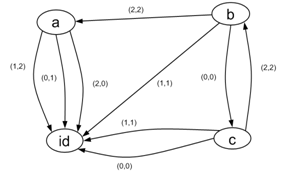
\includegraphics[scale=0.9]{aaronautomaton.png}
\end{center}

We will denote this group $\mathcal{Z}$.   $\mathcal{Z}=\left\langle a,b,c\right\rangle$, where $a,\;b$, and $c$ are defined by the equations:
\begin{align*}
& a=(012)\\ 
& b=(c,1,a)\\
& c=(1,1,b)
\end{align*}

The following identities stem from the generating set of $\mathcal{Z}$:
\begin{align*}
& a^3=b^3=c^3=id\\
& \left|ac\right|=\left|ca\right|=9\\
& \left|ab\right|=\left|ba\right|=27\\
& \left|bc\right|=\left|cb\right|=27\\
\end{align*}

We will use the weight system defined by Bux-P\'{e}rez to try and prove $\mathcal{Z}$ has sub exponential growth.  Using this method we want to ensure that every group element is represented by minimum length words that alternate between $a$'s and/or $a^{-1}$'s and the other generators.  We also need that our elements do not increase in length when split into triplet notation.  Let $\xi=(x_0,x_1,x_2)$ represent any element in $\mathcal{Z}_1$.   In order to analyze the length of elements in $\mathcal{Z}_1$ in triplet form we will use the homomorphism 
\begin{align*}
&(\phi_0,\phi_1,\phi_2):\mathcal{Z}_1\rightarrow \mathcal{Z}\times\mathcal{Z}\times\mathcal{Z}
\end{align*}
where $\phi_0(\xi)=x_0,\;\phi_1(\xi)=x_1$, and $\phi_2(\xi)=x_2$.  Letting $\ell$ represent our length function, $\epsilon\in\left\{-1,1\right\}$, and $\sigma\in\left\langle b,c\right\rangle$, we see that in order for the length of any group element to not increase when split into triplet notation, the following inequality must hold:
\begin{align*}
& \ell(a^{\epsilon})+\ell(\sigma)\geq\ell(\phi_0(\sigma))+\ell(\phi_1(\sigma))+\ell(\phi_2(\sigma))
\end{align*}

The weight of any word is the sum of the weights of the generators that define it.  In order to find weights for $a,\;b$, and $c$ consider the elements $b$, $cbc$, and $(bc)^2$.  Applying the above inequality to $b$ and $cbc$ we get:
\begin{align*}
 \ell(a^{\epsilon})+\ell(b)&\geq\ell(c)+\ell(1)+\ell(a)\Leftrightarrow\\
 \ell(b)&\geq\ell(c)\\
 \ell(a^{\epsilon})+\ell(cbc)&\geq\ell(c)+\ell(1)+\ell(bab)\Leftrightarrow\\
 \ell(a^{\epsilon})+\ell(c)+\ell(b)+\ell(c)&\geq\ell(c)+\ell(b)+\ell(a)+\ell(b)\Leftrightarrow\\
 \ell(c)&\geq\ell(b)
\end{align*}
So we see that the weights of $b$ and $c$ must be equal.  Applying the above inequality to $(bc)^2$ we get:  
%double tailed arrows
\begin{align*}
 \ell(a^{\epsilon})+\ell(bcbc)&\geq\ell(c)+\ell(1)+\ell(abab)\Leftrightarrow\\
 \ell(a^{\epsilon})+\ell(b)+\ell(c)+\ell(b)+\ell(c)&\geq\ell(c)+\ell(1)+\ell(a)+\ell(b)+\ell(a)+\ell(b)\Leftrightarrow\\
 \ell(b)&\geq\ell(a)
\end{align*}
Therefore $a\leq b=c$. We will choose the weights:
\begin{align*}
& \ell(a)=q, &\ell(b)=p,\hspace{2cm} &\ell(c)=p
\end{align*}
Assume $p>q$.  We will choose to define words $\sigma_b\in\left\langle b,c\right\rangle$ as bad if they follow the equality 
\begin{align*}
\ell(a^{\epsilon})+\ell(\sigma)=\ell(\phi_0(\sigma))+\ell(\phi_1(\sigma))+\ell(\phi_2(\sigma))
\end{align*}

\begin{claim}
Any word with only one $b^{\epsilon_n}$ will be bad.
\end{claim}

\begin{proof}
Notice that by our definition of a bad word, the ratio of the weight of some any word $\sigma_b$ plus some $a^{\epsilon_n}$ and the weight of its triple form is going to be $1$.  So any good word $\sigma_g$ must satisfy the following inequality:   
\begin{align*}
& \frac{\ell(\phi_0(\sigma_g))+\ell(\phi_1(\sigma_g))+\ell(\phi_2(\sigma_g))}{\ell(a^{\epsilon})+\ell(\sigma_g)}<1
\end{align*}
It can easily be checked that $c^{\epsilon_n}$ is a good word.  Let us now analyze words of the form $b^{\epsilon_1}c^{\epsilon_2}$.  This word will have the triple form $(c^{\epsilon_1},1,a^{\epsilon_1}b^{\epsilon_2})$ Where $\epsilon_n\in\left\{-1,1\right\}$.  It can easily be seen that any word of this form will be bad.  By adding another $b^{\epsilon_3}$ to this word we are adding $p$ to its weight, thus $\ell(b^{\epsilon_1}c^{\epsilon_2}b^{\epsilon_3})=\ell(b^{\epsilon_1}c^{\epsilon_2})+p$.  Looking at $\phi_0(b^{\epsilon_1}c^{\epsilon_2}b^{\epsilon_3})$ we get $c^{\epsilon_1}c^{\epsilon_3}$, which is simply $c^{\theta_1}$, where $\theta_n\in\left\{-1,0,1\right\}$.  This means that either $\ell(\phi_0(b^{\epsilon_1}c^{\epsilon_2}b^{\epsilon_3}))=\ell(\phi_0(b^{\epsilon_1}c^{\epsilon_2}))$ or  $\ell(\phi_0(b^{\epsilon_1}c^{\epsilon_2}b^{\epsilon_3}))=\ell(\phi_0(b^{\epsilon_1}c^{\epsilon_2}))-p$, depending on what $c^{\epsilon_1}$ and $c^{\epsilon_3}$ are.  Since $\phi_1$ of any element of $\left\langle b,c\right\rangle$ is always the identity, whenever any $b^{\epsilon_n}$ or $c^{\epsilon_n}$ is added to any of these words $\ell(\phi_1)$ of that word is always $0$.  Now, looking at $\phi_2(b^{\epsilon_1}c^{\epsilon_2}b^{\epsilon_3})$ we get $a^{\epsilon_1}b^{\epsilon_2}a^{\epsilon_3}$. We see that $\ell(\phi_2(b^{\epsilon_1}c^{\epsilon_2}b^{\epsilon_3}))=\ell(\phi_2(b^{\epsilon_1}c^{\epsilon_2}))+q$.  Therefore the length of the new word will increase by $p$ while the length of the new word's triple will increase by $q$ or decrease by $p-q$ depending on $c^{\theta_1}$'s.  If this new word's triple increases by $q$ then we will have that $\theta_1\in\left\{-1,1\right\}$, but if it decreases by $p-q$ we will have that $\theta_1=0$ or, in other words, the identity.  We see that the ratio of the weight of $b^{\epsilon_1}c^{\epsilon_2}b^{\epsilon_3}$ and its triple is $\frac{2q+p}{3p+q}$ or $\frac{2q+2p}{3p+q}$ depending on $c^{\theta_1}$.  In either case $b^{\epsilon_1}c^{\epsilon_2}b^{\epsilon_3}$ is good.

Now we have a word of the form $b^{\epsilon_1}c^{\epsilon_2}b^{\epsilon_3}$.  By adding a $c^{\epsilon_4}$ to this word we see that we once again add $p$ to the weight of $b^{\epsilon_1}c^{\epsilon_2}b^{\epsilon_3}$, thus  $\ell(b^{\epsilon_1}c^{\epsilon_2}b^{\epsilon_3}c^{\epsilon_4})=\ell(b^{\epsilon_1}c^{\epsilon_2}b^{\epsilon_3})+p$.  Since $c^{\epsilon_4}=(1,1,b^{\epsilon_4})$, we see that $\ell(\phi_0(b^{\epsilon_1}c^{\epsilon_2}b^{\epsilon_3}c^{\epsilon_4}))=\ell(\phi_0(b^{\epsilon_1}c^{\epsilon_2}b^{\epsilon_3}))$ and $\ell(\phi_1(b^{\epsilon_1}c^{\epsilon_2}b^{\epsilon_3}c^{\epsilon_4}))=\ell(\phi_1(b^{\epsilon_1}c^{\epsilon_2}b^{\epsilon_3}))$.  In $\phi_2(b^{\epsilon_1}c^{\epsilon_2}b^{\epsilon_3}c^{\epsilon_4})$ we will now have $a^{\epsilon_1}b^{\epsilon_2}a^{\epsilon_3}b^{\epsilon_4}$ so $\ell(\phi_2(b^{\epsilon_1}c^{\epsilon_2}b^{\epsilon_3}c^{\epsilon_4}))=\ell(\phi_2(b^{\epsilon_1}c^{\epsilon_2}b^{\epsilon_3}))+p$, therefore the total weight added to the new word's triplet form is just $p$.     We see that the ratio of the weight of $b^{\epsilon_1}c^{\epsilon_2}b^{\epsilon_3}c^{\epsilon_4}$ and its triple is $\frac{2q+2p}{4p+q}$ or $\frac{3p+2q}{4p+q}$ depending on $c^{\theta_1}$.  In either case $b^{\epsilon_1}c^{\epsilon_2}b^{\epsilon_3}c^{\epsilon_4}$ is good.  Notice that when adding a $c^{\epsilon_n}$ to any string of alternating $b^{\epsilon_n}$'s and $c^{\epsilon_n}$'s ending with a $b^{\epsilon_n}$ it adds the same amount of weight to the word and its triple.  This is due to $c^{\epsilon_n}$ only adding weight to $\ell(\phi_2)$ by adding a $b^{\epsilon_n}$ to a string of alternating $b^{\epsilon_n}$'s and $a^{\epsilon_n}$'s.  We see that because $\ell(c^{\epsilon_n})=\ell(b^{\epsilon_n})$ and $b^{\epsilon_n}$ is the only element in the triplet form of $c^{\epsilon_n}$, adding a $c^{\epsilon_n}$ to any word $\sigma$ of alternating $b^{\epsilon_n}$'s and $c^{\epsilon_n}$'s will only add $p$ to $\ell(a^{\epsilon})+\ell(\sigma)$ and $p$ to $\ell(\phi_0(\sigma))+\ell(\phi_1(\sigma))+\ell(\phi_2(\sigma))$.  This means that $c^{\epsilon_n}$ never changes a word from good to bad or bad to good since it can never make the fraction:  
\begin{align*}
& \frac{\ell(\phi_0(\sigma))+\ell(\phi_1(\sigma))+\ell(\phi_2(\sigma))}{\ell(a^{\epsilon})+\ell(\sigma)}=R(\sigma)
\end{align*}
change from being less than one to greater than one or from being greater than one to less than one.

We now have a word of the form $b^{\epsilon_1}c^{\epsilon_2}b^{\epsilon_3}c^{\epsilon_4}=(c^{\theta_1},1,a^{\epsilon_1}b^{\epsilon_2}a^{\epsilon_3}b^{\epsilon_4})$.  Adding some $b^{\epsilon_5}=(c^{\epsilon_5},1,a^{\epsilon_5})$ to this string will once again add $q$ to $\ell(\phi_2(b^{\epsilon_1}c^{\epsilon_2}b^{\epsilon_3}c^{\epsilon_4}))$, do nothing to $\ell(\phi_1(b^{\epsilon_1}c^{\epsilon_2}b^{\epsilon_3}c^{\epsilon_4}))$, and, depending on $c^{\theta_1}$ and $c^{\epsilon_5}$, either increase $\ell(\phi_3(b^{\epsilon_1}c^{\epsilon_2}b^{\epsilon_3}c^{\epsilon_4}))$ by $q$, decrease it by $p$, or keep it the same. If $\epsilon_5=\theta_1\neq0$ or $\epsilon_5\neq\theta_1=0$ then the ratio of the weight of $b^{\epsilon_1}c^{\epsilon_2}b^{\epsilon_3}c^{\epsilon_4}b^{\epsilon_5}$ plus the weight of $a^{\epsilon}$ and its triple is $\frac{3q+3p}{5p+q}$. If $\epsilon_5\neq\theta_1\neq0$ then the ratio of the weight of $b^{\epsilon_1}c^{\epsilon_2}b^{\epsilon_3}c^{\epsilon_4}b^{\epsilon_5}$ plus the weight of $a^{\epsilon}$ and its triple is $\frac{2p+3q}{5p+q}$.  In any of these cases, $b^{\epsilon_1}c^{\epsilon_2}b^{\epsilon_3}c^{\epsilon_4}b^{\epsilon_5}$ is good.  We will consider the worst case scenario of $R(\sigma)$ to be when the $c^{\theta_n}$ in $\phi_0(\sigma)$ is not the identity.  Following this pattern, we see that the worst case scenario of $R(\sigma)$ for some $k$ number of $b^{\epsilon_n}c^{\epsilon_n}$'s will have the form $\frac{p+k(p+q)}{q+k(2p)}$. By adding a $c^{\epsilon_n}$ to the beginning or a $b^{\epsilon_n}$ to the end of those $k$ number of $b^{\epsilon_n}c^{\epsilon_n}$'s, $R(\sigma)$ will have the form $\frac{2p+k(p+q)}{p+q+k(2p)}$ or $\frac{p+q+k(p+q)}{p+q+k(2p)}$ respectively. Thus, we have the equations: 
\begin{align*}
& R((b^{\epsilon_n}c^{\epsilon_n})^k)=\frac{p+k(p+q)}{q+k(2p)}\\
& R(c^{\epsilon_n}(b^{\epsilon_n}c^{\epsilon_n})^k)=\frac{2p+k(p+q)}{p+q+k(2p)}\\
& R((b^{\epsilon_n}c^{\epsilon_n})^kb^{\epsilon_n})=\frac{p+q+k(p+q)}{p+q+k(2p)}
\end{align*}
As $k$ approaches infinity we see that all three of these equations approach $\frac{(p+q)}{(2p)}$, which is clearly less than $1$.  Therefore, for any $k\geq2$ we see that $R((b^{\epsilon_n}c^{\epsilon_n})^k)<1$, $R(c^{\epsilon_n}(b^{\epsilon_n}c^{\epsilon_n})^k)<1$, and $((b^{\epsilon_n}c^{\epsilon_n})^kb^{\epsilon_n})<1$.  Therefore any words of the form $(b^{\epsilon_n}c^{\epsilon_n})^k$, $c^{\epsilon_n}((b^{\epsilon_n}c^{\epsilon_n})^k)$, or $(b^{\epsilon_n}c^{\epsilon_n})b^{\epsilon_n}$ will be good.  For $k\in\left\{0,1\right\}$, the only words that will be bad are words of the form $b^{\epsilon_n}c^{\epsilon_n}$, $c^{\epsilon_n}b^{\epsilon_n}c^{\epsilon_n}$, or $b^{\epsilon_n}$.  It is trivial to check that words of the form $c^{\epsilon_n}b^{\epsilon_n}$ are also bad.  Therefore words with only one $b^{\epsilon_n}$ are bad. If $p=q$ we see that every worst case scenario for $R(\sigma)$ will be equal to $1$ thus making all of the worst case schenario words bad, vastly increasing our number of bad words.  We need a minimal case of bad words so we will only look at the case where $p>q$.
\end{proof}  

This means our list of bad words is:\\

\begin{center}
\begin{tabular}{l | c | c | r }
Word & triple & Word & triple\\
$b$ & $(c,1,a)$ & $b^{-1}$ & $(c^{-1},1,a^{-1})$\\
$bc$ & $(c,1,ab)$ & $b^{-1}c$ & $(c^{-1},1,a^{-1}b)$\\
$bc^{-1}$ & $(c,1,ab^{-1})$ & $b^{-1}c^{-1}$ & $(c^{-1},1,a^{-1}b^{-1})$\\
$c^{-1}b$ & $(c,1,b^{-1}a)$ & $c^{-1}b^{-1}$ & $(c^{-1},1,b^{-1}a^{-1})$\\
$cb$ & $(c,1,ba)$ & $cb^{-1}$ & $(c^{-1},1,ba^{-1})$\\
$cbc$ & $(c,1,bab)$ & $cb^{-1}c$ & $(c^{-1},1,ba^{-1}b)$\\
$c^{-1}bc$ & $(c,1,b^{-1}ab)$ & $c^{-1}b^{-1}c$ & $(c^{-1},1,b^{-1}a^{-1}b)$\\
$c^{-1}bc^{-1}$ & $c,1,b^{-1}ab^{-1})$ & $cb^{-1}c^{-1}$ & $(c^{-1},1,ba^{-1}b^{-1})$\\
$cbc^{-1}$ & $(c,1,bab^{-1})$ & $c^{-1}b^{-1}c^{-1}$ & $(c^{-1},1,b^{-1}a^{-1}b^{-1})$\\
\end{tabular}\\
\end{center}

We see that any bad word has the form $\Psi_\alpha=(c^{\epsilon_n},1,\psi_\alpha)$, Where $\Psi_\alpha$ is any bad element of $\mathcal{Z}$, $\epsilon_n\in\left\{-1,1\right\}$, and $\psi_\alpha\in\left\langle a,b\right\rangle$ is the word of alternating $a^{\epsilon_n}$'s and $b^{\epsilon_n}$'s that correspond to $\Psi_\alpha$.  

\begin{conjecture}
For this generating set, there is no finite primitive set $\mathcal{S}$ for the group $\mathcal{Z}$ such that the number of $\mathcal{S}$-bad blocks of a given length is bounded by some constant independent of the length.
\end{conjecture}

To support this conjecture we will illustrate the process of finding the primitive set, $\mathcal{S}$, of $\mathcal{Z}$. We will use this general form to analyze these bad words.  In attempting to find our primitive set we must find patterns of bad words that either reduce or give good words when split.  This is analogous to the process for finding the primitive sets for $\mathcal{A}$ and $\mathcal{B}$. We want to look at repeated and alternating strings of $a\Psi_\alpha$ and $a^{-1}\Psi_\beta$ and, where $\Psi_\alpha,\Psi_\beta\in\mathcal{Z}_b$. 
 
Case I:

We will first analyze the case where we have a switch from $a^{-1}$'s to $a$'s in some string of alternating $a^{\epsilon}$ and bad words.  Notice that in the area of a string where such a switch occurs we will have $a^\epsilon\Psi_1a^{-1}\Psi_2a\Psi_3$. This $a^\epsilon\Psi_1a^{-1}\Psi_2a\Psi_3=a^\epsilon(c^{\epsilon_1},1,\psi_1)(1,\psi_2,c^{\epsilon_2})(c^{\epsilon_3},1,\psi_3)$ and when multiplying the triples out we get $a^\epsilon(c^{\theta_1},\psi_2,\psi_1\psi_3)$.  Since $c^{\epsilon_1}c^{\epsilon_3}$ multiplies to form a single $c^{\theta_1}$, we see that we have reduction on the second level.  Therefore any string of alternating $a^\epsilon$'s and bad words that contains a switch from an $a^{-1}$ and a bad word to an $a$ and a bad word will have reduction on the second level.

Case II:

We will now analyze the case where there are no switches from $a$ to $a^{-1}$ and vice versa.  We are able to see that for some $m\in\left\{0,1,2,\ldots\right\}$ that any string of $a\Pi_{\alpha_m}$ will have one of the following forms:
\begin{align*}
& \prod^{3m}_{i=1}(a\Psi_{\alpha_i})=[U,V,W]\\
& \prod^{3m+1}_{i=1}(a\Psi_{\alpha_i})=\left[U\psi_{\alpha_{(3m+1)}},Vc^{\epsilon_{(3m+1)}},W\right]a\\
& \prod^{3m+2}_{i=1}(a\Psi_{\alpha_i})=\left[U\psi_{\alpha_{(3m+1)}},Vc^{\epsilon_{(3m+1)}}\psi_{\alpha_{(3m+2)}},Wc^{\epsilon_{(3m+2)}}\right]a^{-1}
\end{align*}
where
\begin{align*}
& U=\prod^{m}_{i=1}(\psi_{\alpha_{(3i-2)}}c^{\epsilon_{(3i)}})\\
& V=\prod^{m}_{i=1}(c^{\epsilon_{(3i-2)}}\psi_{\alpha_{(3i-1)}})\\ 
& W=\prod^{m}_{i=1}(c^{\epsilon_{(3i-1)}}\psi_{\alpha_{(3i)}}) 
\end{align*}
We are also able to see that for some $n\in\left\{0,1,2,\ldots\right\}$ that any string of $a^{-1}\Pi_{\beta_n}$ will have one of the following forms:
\begin{align*}
& \prod^{3n}_{j=1}(a^{-1}\Psi_{\beta_j})=\left[U',V',W'\right]\\
& \prod^{3n+1}_{j=1}(a^{-1}\Psi_{\beta_j})=\left[U',V'\psi_{\beta_{(3m+1)}},W'c^{\epsilon_{(3m+1)}}\right]a^{-1}\\
& \prod^{3n+2}_{j=1}(a^{-1}\Psi_{\beta_j})=\left[U'\psi_{\beta_{(3m+2)}},V'\psi_{\beta_{(3m+1)}}c^{\epsilon_{(3m+2)}},W'c^{\epsilon_{(3m+1)}}\right]a
\end{align*}
where
\begin{align*}
& U^{'}=\prod^{n}_{j=1}(\psi_{\beta_{(3j-1)}}c^{\epsilon_{(3j)}})\\
& V^{'}=\prod^{n}_{j=1}(\psi_{\beta_{(3j-2)}}c^{\epsilon_{(3j-1)}})\\ 
& W^{'}=\prod^{n}_{j=1}(c^{\epsilon_{(3j-2)}}\psi_{\beta_{(3j)}}) 
\end{align*}
For either case, there is no way to get reduction on the second level.  There are, however, ways to produce good generators on the second level.  It can be seen that the only way to produce good generators in either case is if adjacent bad words make an $ab^{\epsilon}c^{\epsilon}b^{\epsilon}a$ or $ac^{\epsilon}a$ on the second level.

Case III:
 
We will now look at the cases where we have a string of alternating $a^\epsilon$'s and bad words that contains a switch from an $a$ and a bad word to an $a^{-1}$ and a bad word.  There are nine possible combinations that can occur depending on where the switch takes place in the string.  These combinations are as follows:
\begin{align*}
& \prod^{3m}_{i=1}(a\Psi_{\alpha_i})\prod^{3n}_{j=1}(a^{-1}\Psi_{\beta_j})=\left[UU',VV',WW'\right]\\
& \prod^{3m}_{i=1}(a\Psi_{\alpha_i})\prod^{3n+1}_{j=1}(a^{-1}\Psi_{\beta_j})=\left[UU',VV'\psi_{\beta_{(3m+1)}},WW'c^{\epsilon_{(3m+1)}}\right]a^{-1}\\
& \prod^{3m}_{i=1}(a\Psi_{\alpha_i})\prod^{3n+2}_{j=1}(a^{-1}\Psi_{\beta_j})=\left[UU'\psi_{\beta_{(3m+2)}},VV'\psi_{\beta_{(3m+1)}}c^{\epsilon_{(3m+2)}},WW'c^{\epsilon_{(3m+1)}}\right]a\\
\\
& \prod^{3m+1}_{i=1}(a\Psi_{\alpha_i})\prod^{3n}_{j=1}(a^{-1}\Psi_{\beta_j})=\left[U\psi_{\alpha_{(3m+1)}}W',Vc^{\epsilon_{(3m+1)}}U',WV'\right]a\\
& \prod^{3m+1}_{i=1}(a\Psi_{\alpha_i})\prod^{3n+1}_{j=1}(a^{-1}\Psi_{\beta_j})=\left[U\psi_{\alpha_{(3m+1)}}W'c^{\epsilon_{(3m+1)}},Vc^{\epsilon_{(3m+1)}}U',WV'\psi_{\beta_{(3m+1)}}\right]\\
& \prod^{3m+1}_{i=1}(a\Psi_{\alpha_i})\prod^{3n+2}_{j=1}(a^{-1}\Psi_{\beta_j})=\left[U\psi_{\alpha_{(3m+1)}}W'c^{\epsilon_{(3m+1)}},Vc^{\epsilon_{(3m+1)}}U'\psi_{\beta_{(3m+2)}},WV'\psi_{\beta_{(3m+1)}}c^{\epsilon_{(3m+2)}}\right]a^{-1}\\
\\
& \prod^{3m+2}_{i=1}(a\Psi_{\alpha_i})\prod^{3n}_{j=1}(a^{-1}\Psi_{\beta_j})=\left[U\psi_{\alpha_{(3m+1)}}V',Vc^{\epsilon_{(3m+1)}}\psi_{\alpha_{(3m+2)}}W'\psi_{\beta_{(3m+1)}},Wc^{\epsilon_{(3m+2)}}U'\right]a^{-1}\\
& \prod^{3m+2}_{i=1}(a\Psi_{\alpha_i})\prod^{3n+1}_{j=1}(a^{-1}\Psi_{\beta_j})=\left[U\psi_{\alpha_{(3m+1)}}V'\psi_{\beta_{(3m+1)}},Vc^{\epsilon_{(3m+1)}}\psi_{\alpha_{(3m+2)}}W'c^{\epsilon_{(3m+1)}},Wc^{\epsilon_{(3m+2)}}U'\right]a\\
& \prod^{3m+2}_{i=1}(a\Psi_{\alpha_i})\prod^{3n+2}_{j=1}(a^{-1}\Psi_{\beta_j})=\left[U\psi_{\alpha_{(3m+1)}}V'\psi_{\beta_{(3m+1)}}c^{\epsilon_{(3m+2)}},Vc^{\epsilon_{(3m+1)}}\psi_{\alpha_{(3m+2)}}W'c^{\epsilon_{(3m+1)}},Wc^{\epsilon_{(3m+2)}}U'\psi_{\beta_{(3m+2)}}\right]
\end{align*}
We can see that there are possibilities for reduction and the production of good generators in the second level of all nine combinations.  This is still only possible through adjacent bad words however.  We see that when defining our primitive set we only need to look at alternating strings of $a^{\epsilon}$'s and bad words that contain only two or less bad words. There are only a finite number of ways to keep pairs of $a^{\epsilon}\Psi$'s bad.  A problem arises when attempting to find all the ways to keep these pairs bad when attaching them to other pairs.  There appears to be an infinite number of ways to attach $a^{-1}\Psi$ pairs to other $a^{-1}\Psi$ pairs without getting reduction or producing a good generator.  Similarly, there also appears to be an infinite number of ways to attach $a\Psi$ pairs to other $a\Psi$ pairs witout getting reduction or producing any good genorators.  Even still there are an infinite number of places to switch from $a\Psi$ pairs to $a^{-1}\Psi$ pairs.  This means that it seems to be impossible to find a finite number of ways to make bad words in order to define our primitive set.

\section{Acknowledgements}

We would like to thank our seminar director, Dr. Daniel Farley, for his guidance and expertise throughout our research. We would also like to thank our graduate assistant, Rachel Karpman, for her support through many long hours and late nights. Our gratitude goes out to all the faculty at Miami University involved in SUMSRI for their contributions and commitment to helping undergraduates. We also thank the National Science Foundation, the National Security Agency, and Miami University for making the research program possible.



%%%%%%%%%%%%%%%%%%%%%%%%%%%%%%%%%%%%%%%%%%%%%%%%%%%%%%%%%%%%%%%%%%%%%%%%%%%%%%%%%%%%%%%%%%%%%%%%%%%



\begin{thebibliography}{999}

\bibitem{Nekr} V. Nekrashevych, {\it Self-Similar Groups}, American Mathematical Society, Providence, RI, 2005.
\bibitem{BuxP} K. Bux, R. P\'{e}rez {\it On the Growth of Iterated Monodromy Groups}, preprint, 2004.
\bibitem{Terp} A. Terpstra {\it The Grigorchuk Group, the Burnside Problem, and Milnor's Question}, unpublished.
\bibitem{Bart} L. Bartholdi, V. Nekrashevych {\it Iterated Monodromy Groups of Quadratic Polynomials, I}, preprint 2006.
\bibitem{Grig} R. Grigorchuck, I Pak, {\it Groups of Intermediate Growth: An Introduction for Beginners}, Enseign. Math. (2) \textbf{54}(2008), no. 3-4, 251-272







\end{thebibliography}
























\end{document}
